%\documentclass[compress,pdftex%draft
%]{beamer}
\documentclass[slidestop,compress,mathserif]{beamer}
%\usepackage[bars]{beamerthemetree} % Beamer theme v 2.2
\usetheme{Berlin} % Beamer theme v 3.0
\usecolortheme{seahorse} % Beamer color theme

\setbeamertemplate{itemize items}[default]
\setbeamertemplate{enumerate items}[default]

\setbeamertemplate{footline}[frame number]

\usepackage{multicol}
\usepackage{amsmath}
\usepackage[retainorgcmds]{IEEEtrantools}

\usepackage{pdfpages}



% \include{highlight.css}

% \usepackage{beamerthemeshadow}

% \usepackage{listings}
% \usepackage{etex}
% %%%%%%%%%%%
% % fonts for listing
% %%%%%%%%%%%
% % \defaultfontfeatures{Scale=MatchLowercase}
% % \setmainfont[Mapping=tex-text]{Georgia}
% % \setsansfont[Mapping=tex-text]{Arial}
% % \setmonofont{Courier New}
% %%%%%%%%%%%
% \usepackage[usenames,dvipsnames]{pstricks}
% \usepackage{epsfig}
% \usepackage{pst-grad} % For gradients
% \usepackage{pst-plot} % For axes
% \usepackage{epstopdf}
% \usepackage{proof}
% \usepackage{calrsfs}
% %\usepackage{ICALPbeamerthemeshadow}
% \usepackage{amsmath,stmaryrd,amssymb,latexsym,rotating}
% \usepackage[latin1]{inputenc}
% \usepackage[english]{babel}
% \usepackage{alltt}
% \usepackage{graphics}
% %\usepackage[cspex]{mathbbol}
% %\usepackage[all]{xy}

% % Try the class options [notes], [notesonly], [trans], [handout],
% % [red], [compress], [draft] and see what happens!

% % Copyright 2003 by Till Tantau <tantau@users.sourceforge.net>.
% %
% % This program can be redistributed and/or modified under the terms
% % of the LaTeX Project Public License Distributed from CTAN
% % archives in directory macros/latex/base/lppl.txt.

% % For a green structure color use:
% \colorlet{structure}{green!50!black}
% \definecolor{ocre}{rgb}{.41,.34,0}
% \definecolor{lightgreen}{rgb}{0.79,0.86,.79}
% \definecolor{lesslightgreen}{rgb}{0.39,.9,.39}
% \definecolor{mydarkgreen}{rgb}{0.10,0.43,0}
% \usetheme{Warsaw}
% \setbeamercovered{dynamic}

% \beamerboxesdeclarecolorscheme{point}{blue}{blue!15!averagebackgroundcolor}
% \beamerboxesdeclarecolorscheme{good}{green}{green!15!averagebackgroundcolor}
% \beamerboxesdeclarecolorscheme{bad}{red}{red!15!averagebackgroundcolor}

% \definecolor{darkgreen}{rgb}{0,0.65,0.08}
% \definecolor{darkblue}{rgb}{0,0.08,0.55}

% define new command
\newcommand{\bdm}
{
\begin{displaymath}
\begin{array}{rcl}
}
\newcommand{\edm}
{
\end{array}
\end{displaymath}
}
\newcommand{\bda}[1]
{
\begin{displaymath}
\begin{array}{#1}
}
\newcommand{\eda}
{
\end{array}
\end{displaymath}
}
\newcommand{\bIm}
{
\begin{IEEEeqnarray}{rCl}
}
\newcommand{\eIm}
{
\end{IEEEeqnarray}
}


\title[Accelerate Reed-solomon coding for Fault-Tolerance in RAID-like system]{Accelerate Reed-solomon coding for Fault-Tolerance in RAID-like system}
\author{Shuai YUAN}
\institute[LSA lab,  NTHU]{
  NTHU \\
  LSA lab}
\date{}
%\ThisCenterWallPaper{1}{inc/cover} % Background Image
\begin{document}

\frame{\titlepage}
\frame{\frametitle{Outline}
\begin{itemize}
\item Background
\item How to use CUDA to accelerate
\item Experiment
\item Q \& A
% \item Appendix
\end{itemize}
}

\section{Background} % Bookmark information
\subsection{Why Reed-Solomon codes?} % Bookmark information
\begin{frame}[options]
\frametitle{Why fault-tolerance?}
In a RAID-like system, storage is distributed among several devices, the probability of one of these devices failing becomes significant. 

\only<2-3>
{
MTTF (mean time to failure) of one device is $P$, 

MTTF of a system of $n$ devices is $\dfrac{P}{n}$.
}

\only<3>
{
Thus in such systems, fault-tolerance must be taken into account.
}
\end{frame}

\begin{frame}[options]
\frametitle{Why erasure codes?}
{\color{blue}{Replication}} is expensive!

e.g. To achieve double-fault tolerance,
we need 2 replicas.


\end{frame}


%\subsection{Erasure Codes} % Bookmark information
\begin{frame}[options]
\frametitle{Erasure Codes}

Given a message/file of $k$ equal-size blocks/chunks/fragments, encode it into $n$ blocks/chunks/fragments ($n > k$)

\begin{itemize}
  \item Optimal erasure codes: any $k$ out of the $n$ fragments are sufficient to recover the original message/file. \\
	i.e. can tolerate arbitrary $(n-k)$ failures. \\
	We call this {\color{red}{(n,k) MDS (maximum distance separable) property}}. \\
	e.g. Reed Solomon Codes
  \item Near-optimal erasure codes: require $( 1 + \varepsilon )k$ code blocks/chunks to recover ($\varepsilon > 0$). \\
	i.e. cannot tolerate arbitrary $(n-k)$ failures. \\
  	e.g. Local Reconstruction Codes (used in WAS)
\end{itemize}

\end{frame}

\begin{frame}[options]
\frametitle{Replication vs. Erasure Codes}

Given a file of size $M$

Using Reed Solomon Codes(n=4, k=2)
\begin{figure}[ht!]
%  \centering
%  \includegraphics[scale=0.28]{R-S-Codes.png}
  \includegraphics[scale=0.4]{pic/RS-2-4.png}
%  \caption{R-S Codes}
%  \label{}
\end{figure}

Achieve double fault tolerance
%, and we only need additional data of size M.
\begin{itemize}
  \item R-S Codes: storage overhead = $M$
  \item Relication: storage overhead = $2M$ (2 replicas)
\end{itemize}
\end{frame}


\subsection{Reed-Solomon coding mechanism}
\begin{frame}[options]
\frametitle{Reed-Solomon encoding process}
\only<1>
{
%Why R-S Codes have MDS property?

%}
%
%\only<>
%{
%More general:

Given file $F$:
divide it into $k$ equal-size native chunks: 
$F = [F_{i}]_{i=1,2,\dots,k}$.
%$(F_{i})_{i=1,2,\dots,k(n-k)}$.
Encode them into $(n-k)$ code chunks: 
$C = [C_{i}]_{i=1,2,\dots,n-k}$.

Use Encoding Matrix $EM_{(n-k) \times k}$ to produce code chunks:
%(Use Vandermonde Matrix) 
\begin{displaymath}
\begin{array}{rcl}
C^{T} &=& EM \times F^{T} 
\end{array}
\end{displaymath}
$C_{i}$ is the linear combination of $F_{1}, F_{2}, \dots, F_{k}$.
}

\only<2>
{
In our case,
\begin{displaymath}
\begin{array}{rcl}
F &=& \begin{pmatrix} A & B \end{pmatrix} \\
EM &=& 	\begin{pmatrix}
		  1 & 1 \\
		  1 & 2 \\
		\end{pmatrix} \\
%C &=& \begin{pmatrix} A & B & A+B & A+2B \end{pmatrix}
C^{T} &=& \begin{pmatrix} 1 & 1 \\  1 & 2 \\ \end{pmatrix} \times \begin{pmatrix} A \\ B \end{pmatrix} \\
&=& \begin{pmatrix} A+B \\ A+2B \end{pmatrix}
\end{array}
\end{displaymath}
}

\only<3>
{

Let $P = [P_{i}]_{i=1,2,\dots,n} = [F_{1}, F_{2}, \dots, F_{k}, C_{1}, C_{2}, \dots, C_{n-k}]$ be the $n$ chunks in storage, 
$EM' = \begin{pmatrix} I \\ EM \end{pmatrix}$,
Here 
$$
I = \begin{pmatrix} 
  1 & 0 & \ldots & 0 \\ 
  0 & 1 & \ldots & 0 \\
  \vdots & \vdots & \ddots & \vdots \\
  0 & 0 & \ldots & 1 
\end{pmatrix}
$$
then
\begin{displaymath}
\begin{array}{rcl}
P^{T} &=& EM' \times F^{T} \\
&=& \begin{pmatrix} F^{T} \\ C^{T} \end{pmatrix}
\end{array}
\end{displaymath}
}

\only<4>
{
In our case,
\begin{displaymath}
\begin{array}{rcl}
EM' &=& \begin{pmatrix} I \\ EM \end{pmatrix} 
  = \begin{pmatrix}
	1 & 0 \\
	0 & 1 \\
	1 & 1 \\
	1 & 2 \\
	\end{pmatrix} \\	
P^{T} &=& EM' \times F^{T} \\
&=& \begin{pmatrix}
	1 & 0 \\
	0 & 1 \\
	1 & 1 \\
	1 & 2 \\
	\end{pmatrix}
	\times
	\begin{pmatrix} A \\ B \end{pmatrix} \\
	&=& \begin{pmatrix}
	A \\
	B \\
	A+B \\
	A+2B
	\end{pmatrix}
\end{array}
\end{displaymath}

}


\only<5>
{
$EM'$ is the key of MDS property!
}

\only<6>
{
\begin{theorem}[necessary and sufficient condition]
  Every possible $k \times k$ submatrix obtained by removing $(n-k)$ rows from $EM'$ has {\color{red}{full rank}}.

equivalent expression of {\color{red}{full rank}}:
\begin{itemize}
  \item rank = $k$
  \item non-singular \\
$\vdots$
\end{itemize}

\end{theorem}

Alternative view:

Consider the linear space of $P = [P_{i}]_{i=1,2,\dots,n} = [F_{1}, F_{2}, \dots, F_{k}, C_{1}, C_{2}, \dots, C_{n-k}]$,
its dimension is $k$, and any $k$ out of $n$ vectors form a basis of the linear space.
}

\only<7>
{
Reed-Solomon Codes uses Vandermonde matrix $V$ as $EM$
$$
V =
\begin{bmatrix}
1 & 1 & 1 & \ldots & 1 \\
1 & 2 & 3 & \ldots & k \\
1^2 & 2^2 & 3^2 & \ldots & k^2 \\
\vdots & \vdots & \vdots & \ddots & \vdots \\
1^{(n-k)} & 2^{(n-k)} & 3^{(n-k)} & \ldots & k^{(n-k)}
\end{bmatrix}
$$
}

\only<8>
{
$$
EM' =
\begin{bmatrix}
1 & 0 & 0 & \ldots & 0 \\
0 & 1 & 0 & \ldots & 0 \\
0 & 0 & 1 & \ldots & 0 \\
\vdots & \vdots & \vdots & \ddots & \vdots \\
0 & 0 & 0 & \ldots & 1 \\
1 & 1 & 1 & \ldots & 1 \\
1 & 2 & 3 & \ldots & k \\
1^2 & 2^2 & 3^2 & \ldots & k^2 \\
\vdots & \vdots & \vdots & \ddots & \vdots \\
1^{(n-k)} & 2^{(n-k)} & 3^{(n-k)} & \ldots & k^{(n-k)}
\end{bmatrix}
$$

}

\only<9>
{
%\begin{displaymath}
%\begin{array}{rcl}
%\textrm{For } i=1,2,\dots,n(n-k) &&\\
%For $i=1,2,\dots,n(n-k)$
%\begin{displaymath}
%\begin{array}{rcl}
%P_{i} &=& ECV_{i} \times F^{T} \\
%&=& \sum_{j=1}^{k(n-k)} \alpha_{i,j}F_{j}
%\end{array}
%\end{displaymath}
%$ECV_{i}$: encoding coeffient vector of $P_{i}$.
Remark:
\begin{itemize}
  \item All arithmetic operations in Galois Field GF($2^{x}$). Then every number is less than $2^{x}$.
%e.g. $+/- \rightarrow xor$
  \item $EM'$ satisfies MDS property.
\end{itemize}

}
\end{frame}


\begin{frame}[options]
\frametitle{Reed-Solomon decoding process}
We randomly select $k$ out of $n$ fragments, say $X = [x_{1}, x_{2}, \cdots, x_{k}]^{T}$.

Then we use the coefficients of each fragments $x_{i}$ to construct a $k \times k$ matrix $V'$.

Original data can be regenerated by multiplying matrix $X$ with the inverse of matrix $V'$:

$$
F = V'^{-1} X 
$$
\end{frame}


\subsection{Optimization motivation}
\begin{frame}[options]
\frametitle{Optimization motivation}
The reason that discourages using Reed-Solomon coding to replace replication is its high computational complexity:
\begin{itemize}
  \item Galois Field arithmetic
  \item matrix operations
\end{itemize}
\end{frame}



\section{How to use CUDA to accelerate} % Bookmark information
\subsection{Accelerate operations in Galois Field (GF)} % Bookmark information
\begin{frame}[options]
\frametitle{Accelerate operations in Galois Field (GF)}
GF($2^w$) field is constructed by finding a primitive polynomial $q(x)$ of degree $w$ over GF(2), and then enumerating the elements (which are polynomials) with the generator $x$.
Addition in this field is performed using polynomial addition, and multiplication is performed using polynomial multiplication and taking the result modulo $q(x)$.

\only<2->
{
In implementation, we
map the elements of GF($2^w$) to binary words of size $w$, so that computation in GF($2^w$) becomes bitwise operations.
Let $r(x)$ be a polynomial in GF($2^w$). Then we can map $r(x)$ to a binary word $b$ of size $w$ by setting the $i$th bit of $b$ to the coefficient of $x^i$ in $r(x)$.
}

\only<3->
{
After mapping, 
Addition/subtraction of binary elements of GF($2^w$) can be performed by bitwise exclusive-or. 
}
\end{frame}

\begin{frame}[options]
\frametitle{Accelerate operations in Galois Field (GF)}
\only<1>
{
However, multiplication is still costly.

Use bitwise operations to emulate polynomial multiplication in GF($2^w$): a loop of $w$ iterations.

e.g. 
In GF($2^8$), multiplying 2 bytes takes 8 iterations.
}

\only<2>
{
\begin{block}{CPU approach}
store all the result in a multiplication table
\end{block}

e.g. 
In GF($2^8$), multiplying 2 bytes takes $256 \times 256=64KB$

consumes a lot of space $\leadsto$ not suitable for GPU
}

\only<3>
{
trade-off between computation and memory consumption (\cite{plank1997tutorial})

We build up two smaller tables:
\begin{itemize}
  \item exponential table: maps from a binary element $b$ to power $j$ such that $x^j$ is equivalent to $b$.
  \item logarithm table: maps from a power $j$ to its binary element $b$ such that $x^j$ is equivalent to $b$.
\end{itemize}

Multiplication in GF($2^w$):
\begin{itemize}
  \item looking each binary number in the logarithm table for its logarithm (this is equivalent to finding the polynomial)
  \item adding the logarithms modulo $2^w-1$ (this is equivalent to multiplying the polynomial modulo $q(x)$)
  \item looking up exponential table to convert the result back to a binary number
\end{itemize}
Totally three table lookups and a modular addition.
}
\end{frame}



\subsection{Accelerate encoding process}
\begin{frame}[options]
\frametitle{Accelerate encoding process}
\begin{itemize}
  \item Generating Vandermonde's Matrix
  \item Matrix multiplication
\end{itemize}
\end{frame}

\subsection{Accelerate decoding process}
\begin{frame}[options]
\frametitle{Accelerate decoding process}
\begin{itemize}
  \item Computing inverse matrix
  \item Matrix multiplication
\end{itemize}
\end{frame}

\begin{frame}[options]
\frametitle{Accelerate matrix inversion}
Guassian/Guass-Jordon elimination in GF($2^8$)
\only<1>
{
$$
[V' I] =
\begin{bmatrix}
1 & 0 & 0 & 0 & | & 1 & 0 & 0 & 0 \\
0 & 1 & 0 & 0 & | & 0 & 1 & 0 & 0 \\
1 & 2 & 3 & 4 & | & 0 & 0 & 1 & 0  \\
1 & 1 & 1 & 1 & | & 0 & 0 & 0 & 1  \\
\end{bmatrix}
$$
}
\only<2>
{
$$
[V' I] =
\begin{bmatrix}
1 & 0 & 0 & 0 & | & 1 & 0 & 0 & 0 \\
0 & 1 & 0 & 0 & | & 0 & 1 & 0 & 0 \\
0 & 2 & 3 & 4 & | & 1 & 0 & 1 & 0  \\
0 & 1 & 1 & 1 & | & 1 & 0 & 0 & 1  \\
\end{bmatrix}
$$
}
\only<3>
{
$$
[V' I] =
\begin{bmatrix}
1 & 0 & 0 & 0 & | & 1 & 0 & 0 & 0 \\
0 & 1 & 0 & 0 & | & 0 & 1 & 0 & 0 \\
0 & 0 & 3 & 4 & | & 1 & 2 & 1 & 0  \\
0 & 0 & 1 & 1 & | & 1 & 1 & 0 & 1  \\
\end{bmatrix}
$$
}
\only<4>
{
$$
[V' I] =
\begin{bmatrix}
1 & 0 & 0 & 0 & | & 1 & 0 & 0 & 0 \\
0 & 1 & 0 & 0 & | & 0 & 1 & 0 & 0 \\
0 & 0 & 1 & 247 & | & 244 & 245 & 244 & 0  \\
0 & 0 & 0 & 246 & | & 245 & 244 & 244 & 1  \\
\end{bmatrix}
$$
}
\only<5>
{
$$
[V' I] =
\begin{bmatrix}
1 & 0 & 0 & 0 & | & 1 & 0 & 0 & 0 \\
0 & 1 & 0 & 0 & | & 0 & 1 & 0 & 0 \\
0 & 0 & 1 & 0 & | & 104 & 187 & 186 & 210  \\
0 & 0 & 0 & 1 & | & 105 & 186 & 186 & 211  \\
\end{bmatrix}
$$
}

\only<6>
{
\begin{block}{GPU}
  \begin{itemize}
	\item normalize row
	\item make column into reduced echelon form
	\end{itemize}
\end{block}
}

\end{frame}

\section{Experiment} % Bookmark information
\subsection{Experiment Settings} % Bookmark information
\begin{frame}[options]
\frametitle{Experiment Settings}
\begin{itemize}
  \item Intel(R) Xeon(R) CPU E5620  @ 2.40GHz
  \item nVidia Corporation GF100 [Tesla C2050]
	\begin{itemize}
	  \item 448 CUDA cores @ 1.15GHz
	  \item 3GB GDDR5 (1.44GB/s)
	  \item 64KB L1 cache + shared memory / 32 cores, 768KB L2 cache
	\end{itemize}
%  \item k=4, n=6 for GPU vs CPU
\end{itemize}
\end{frame}
\subsection{Experiment Result (GPU vs CPU)} % Bookmark information
\begin{frame}[options]
\frametitle{Experiment Result (fixed $n,k$)}
\only<1-2>
{
$k = 4, n = 6$
}
\only<1>
{
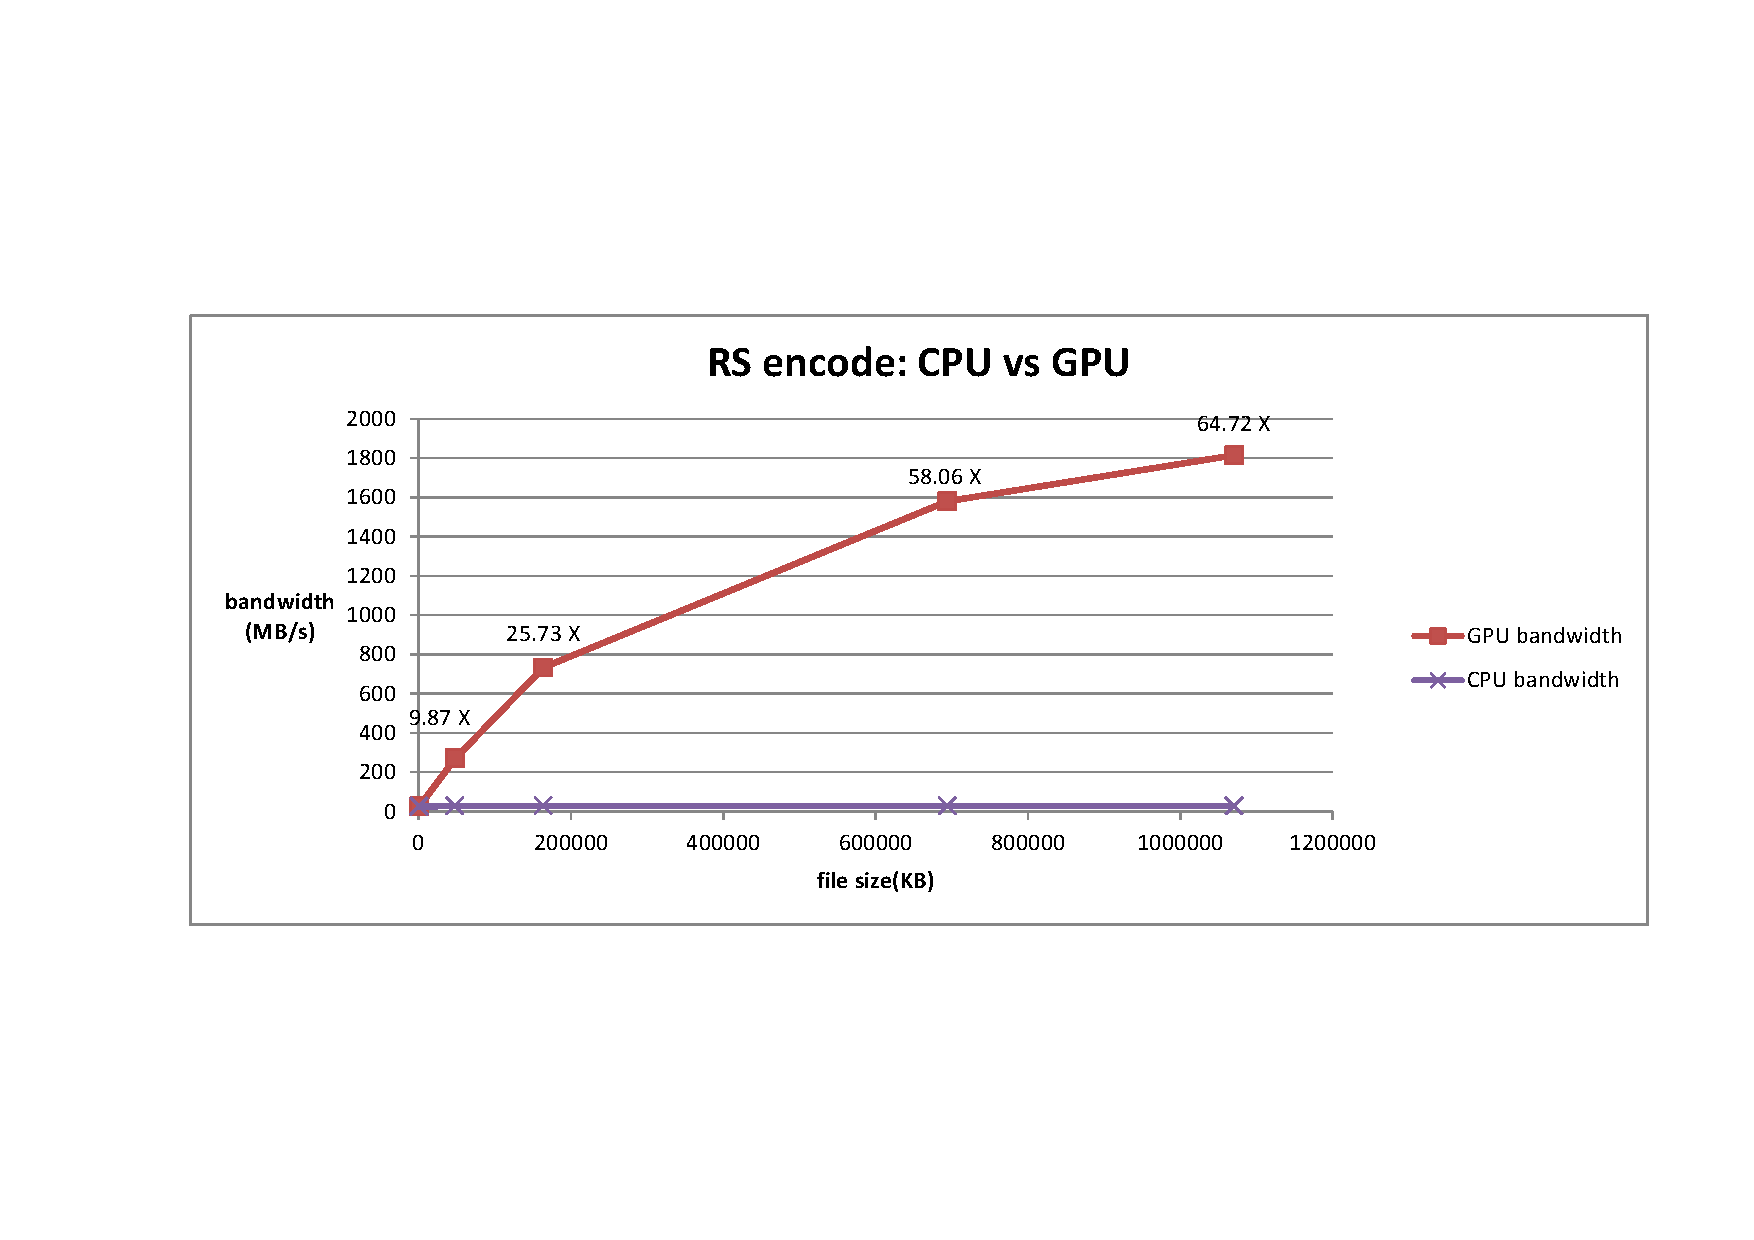
\includegraphics[scale=0.46]{../result-graph/encode-CPU-vs-GPU-graph.pdf}

}
\only<2>
{
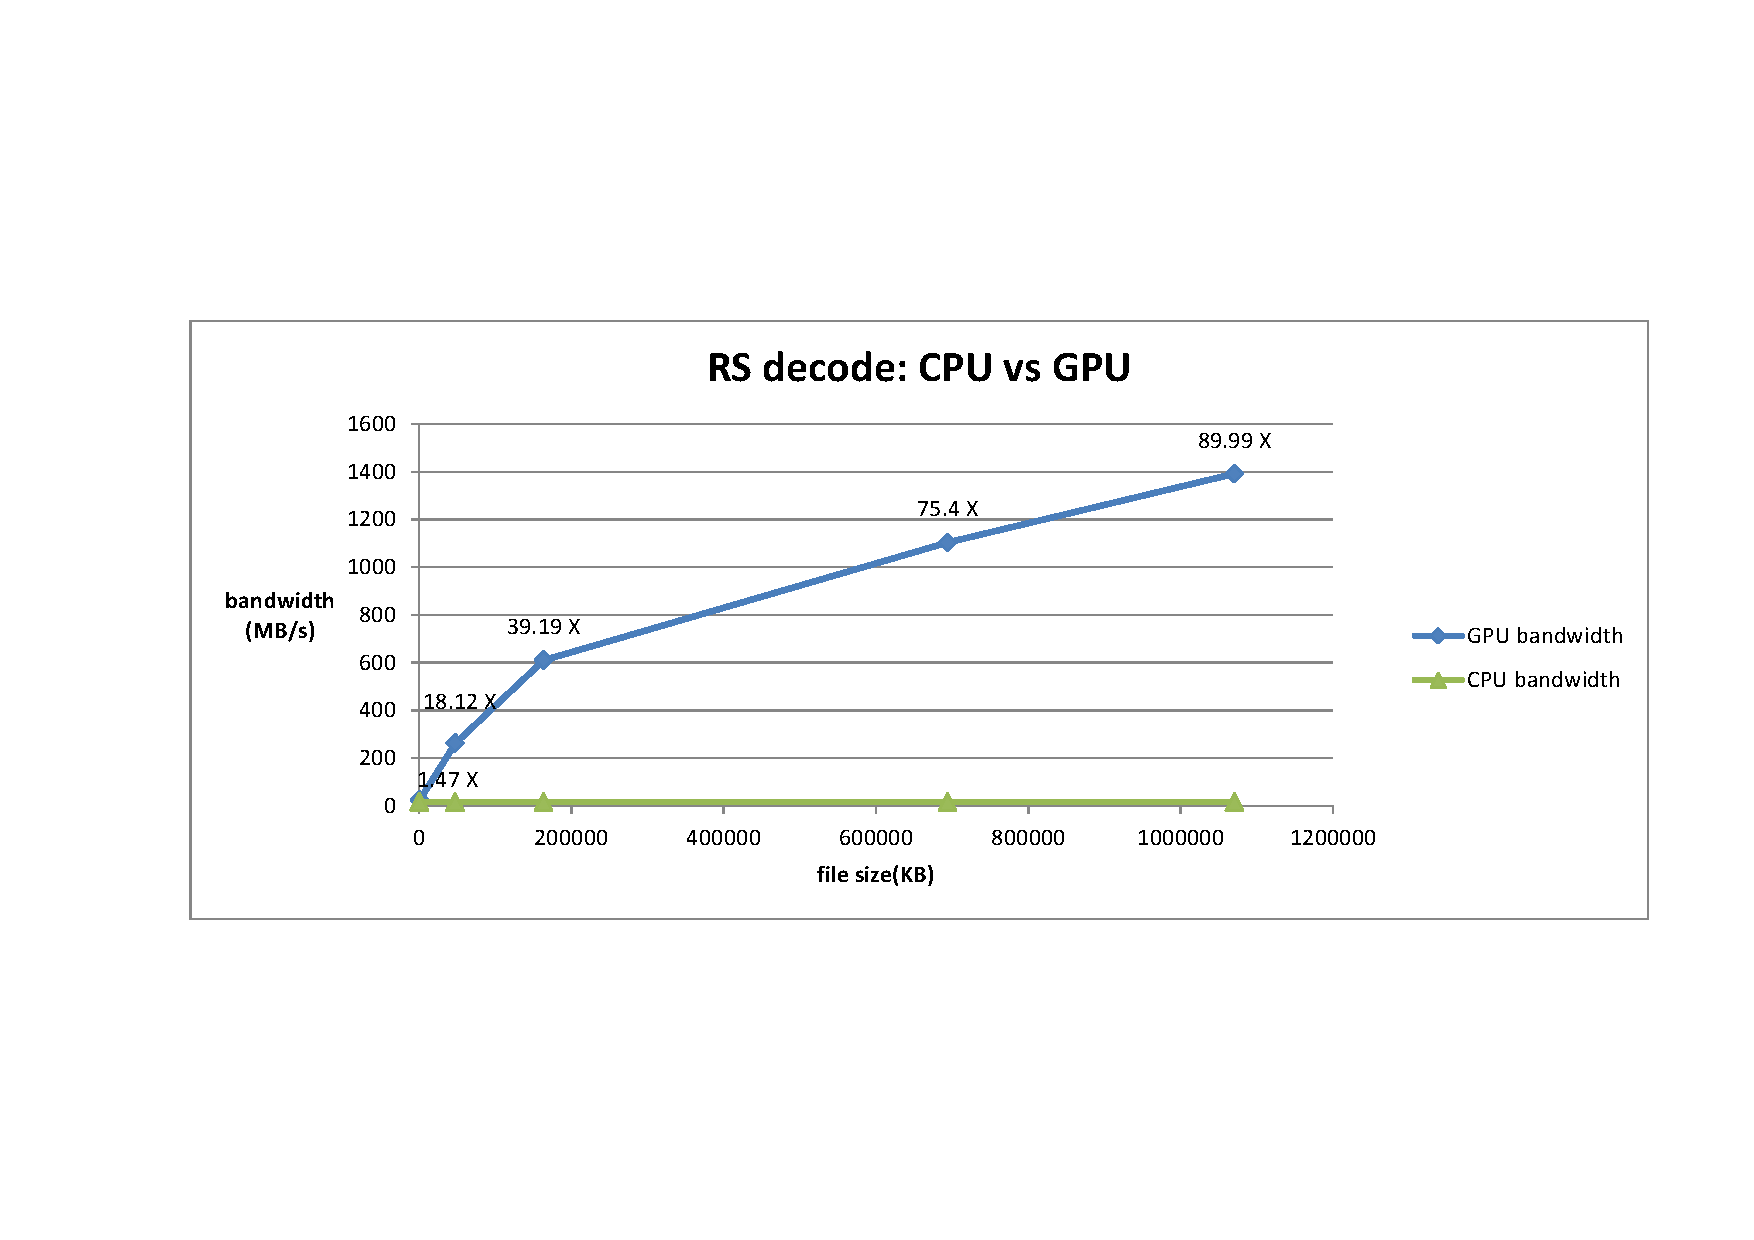
\includegraphics[scale=0.46]{../result-graph/decode-CPU-vs-GPU-graph.pdf}
}
\only<3>
{
\begin{block}{Conclusion}
\begin{enumerate}
\item CPU bandwidth is nearly constant.
\item GPU achieves better speed-up when the file size scales up.
\item GPU performance speed-up gets slower.
\end{enumerate}
\end{block}
}
\end{frame}

%\subsection{tuning k} % Bookmark information
\begin{frame}[options]
%\frametitle{Experiment Result (tuning k)}
\frametitle{Experiment Result (fixed file size)}
\only<1-8>
{
File size: 1.1GB
}

\only<1-4>
{
double fault tolerance	
}
\only<5-8>
{
triple fault tolerance	
}
\only<1>
{
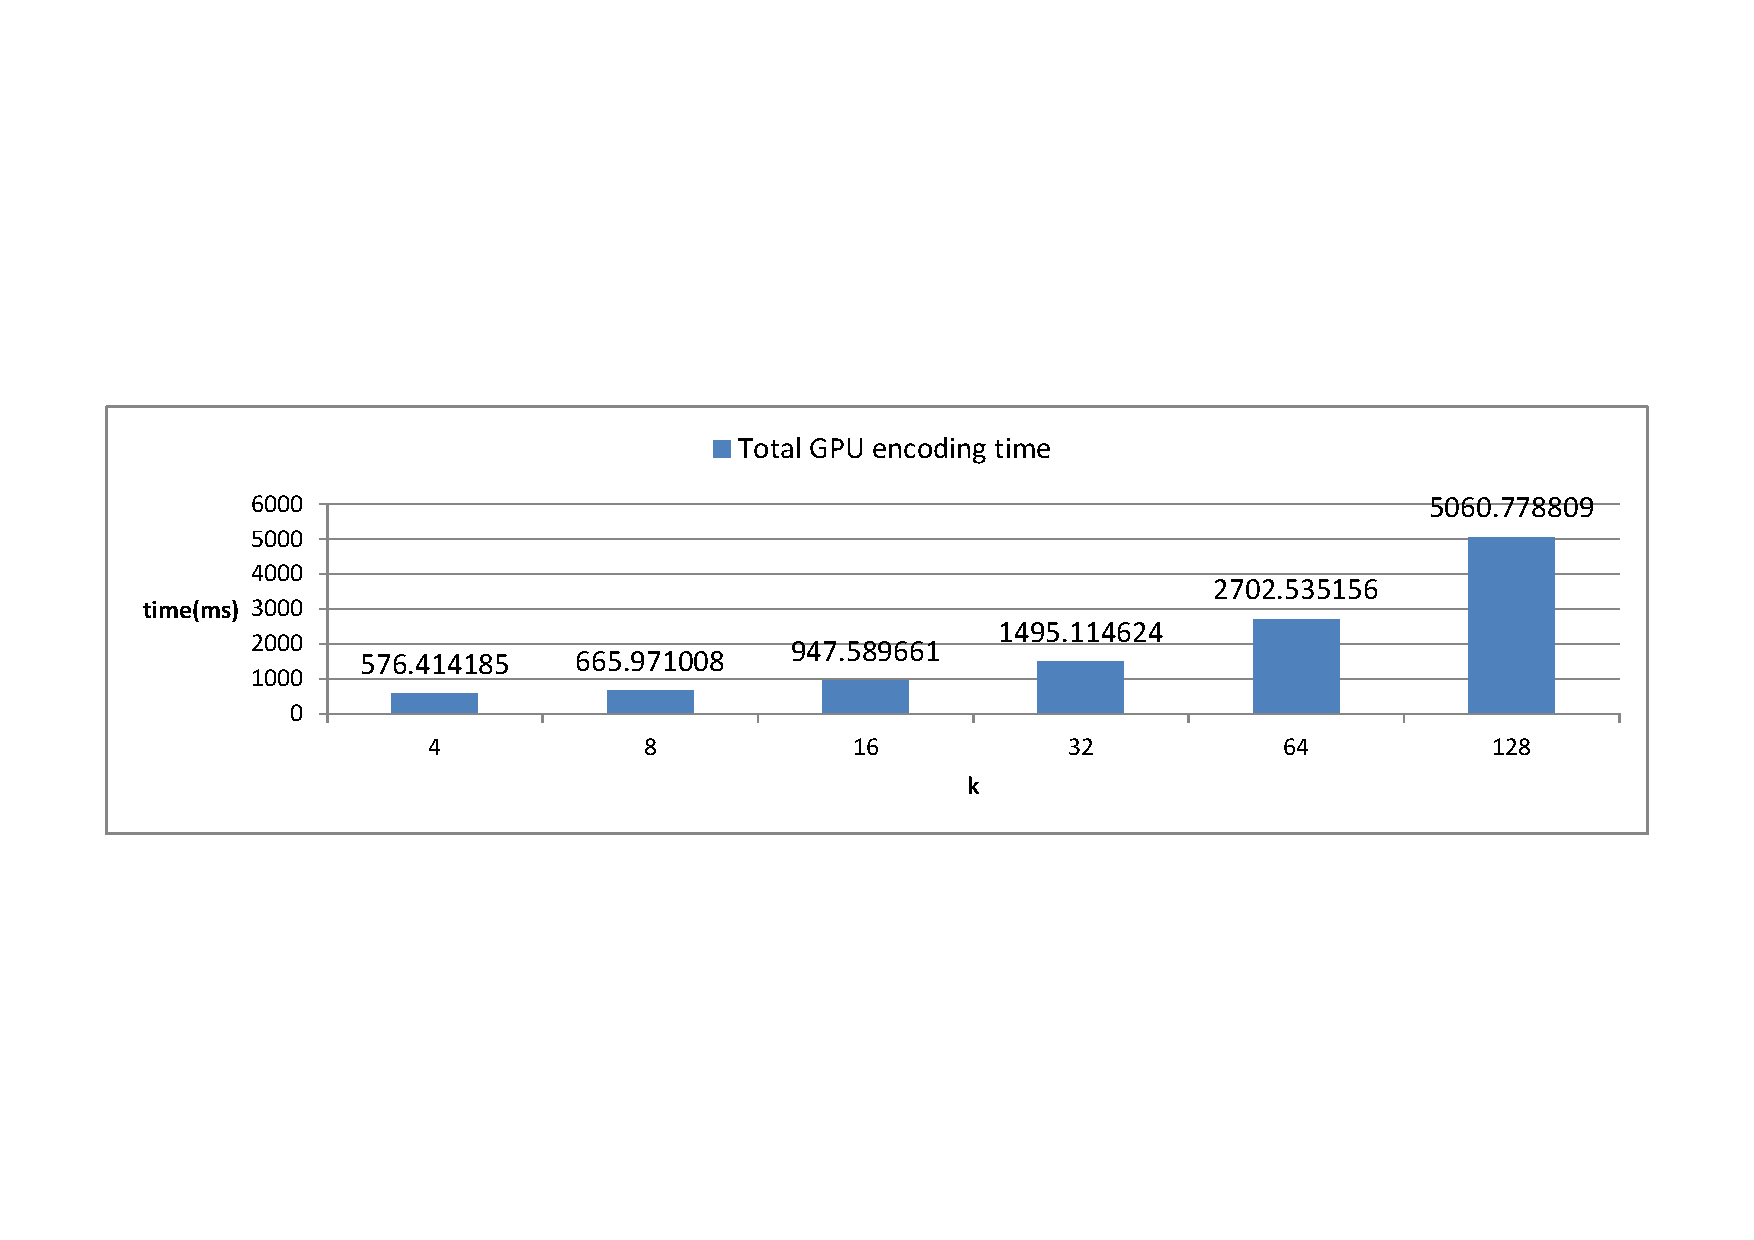
\includegraphics[scale=0.42]{../result-graph/Total-GPU-encoding-time-2.pdf}
}
\only<2>
{
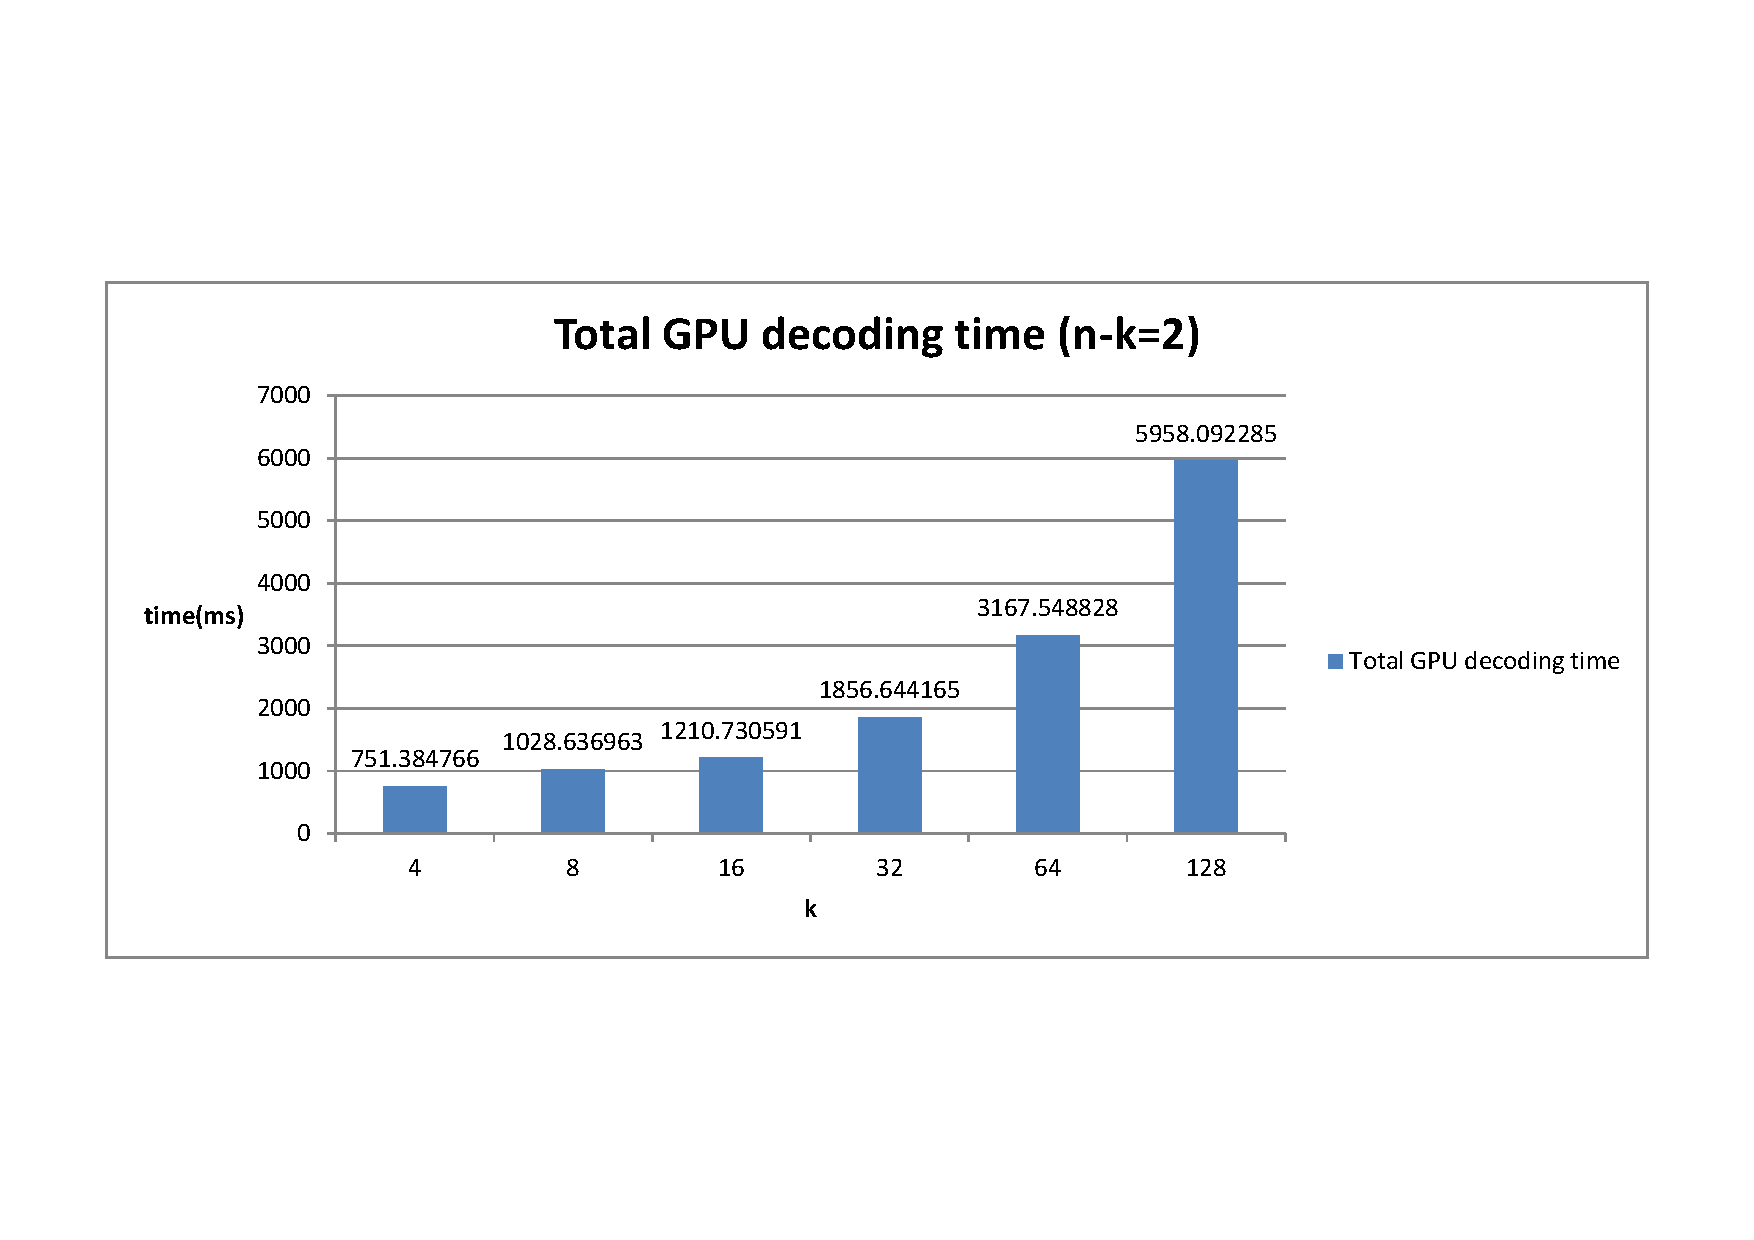
\includegraphics[scale=0.42]{../result-graph/Total-GPU-decoding-time-2.pdf}
}
\only<3>
{
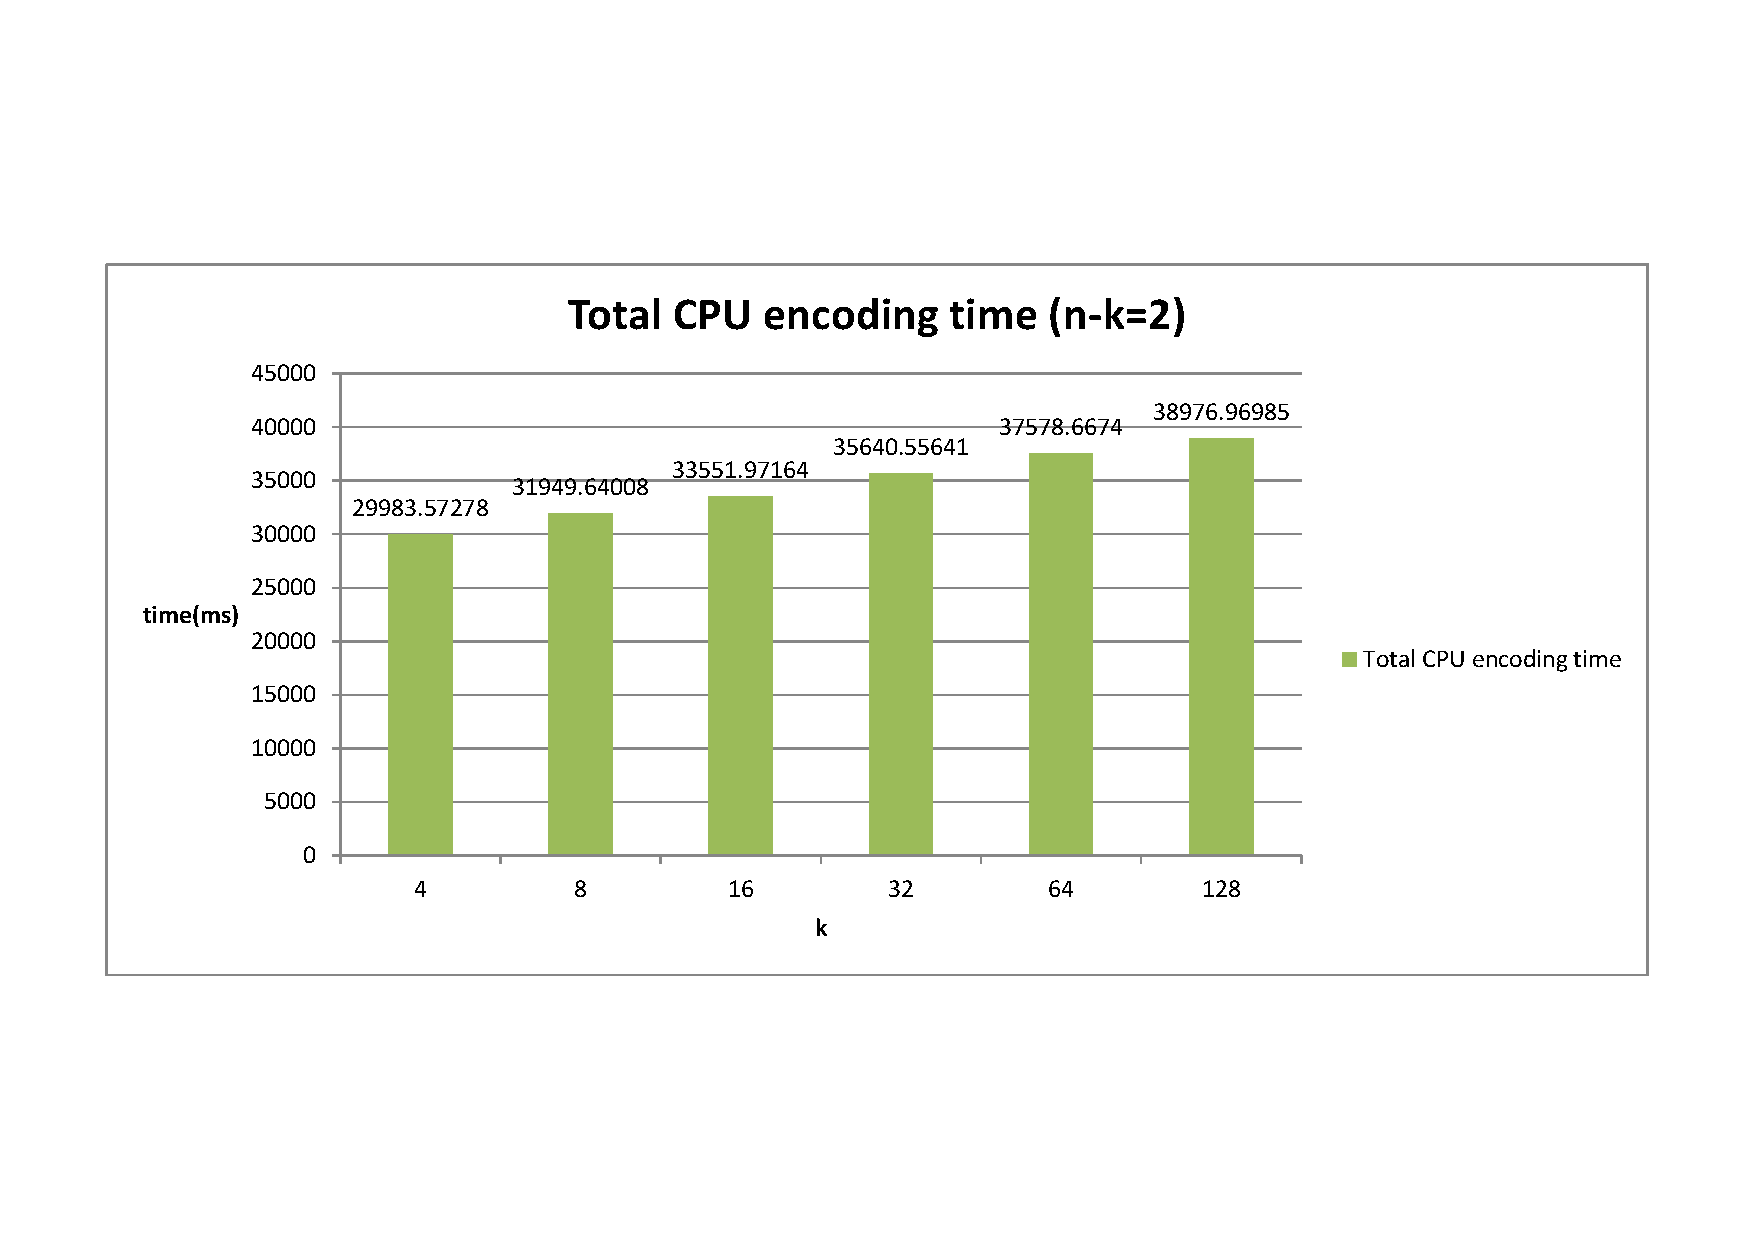
\includegraphics[scale=0.42]{../result-graph/Total-CPU-encoding-time-2.pdf}
}
\only<4>
{
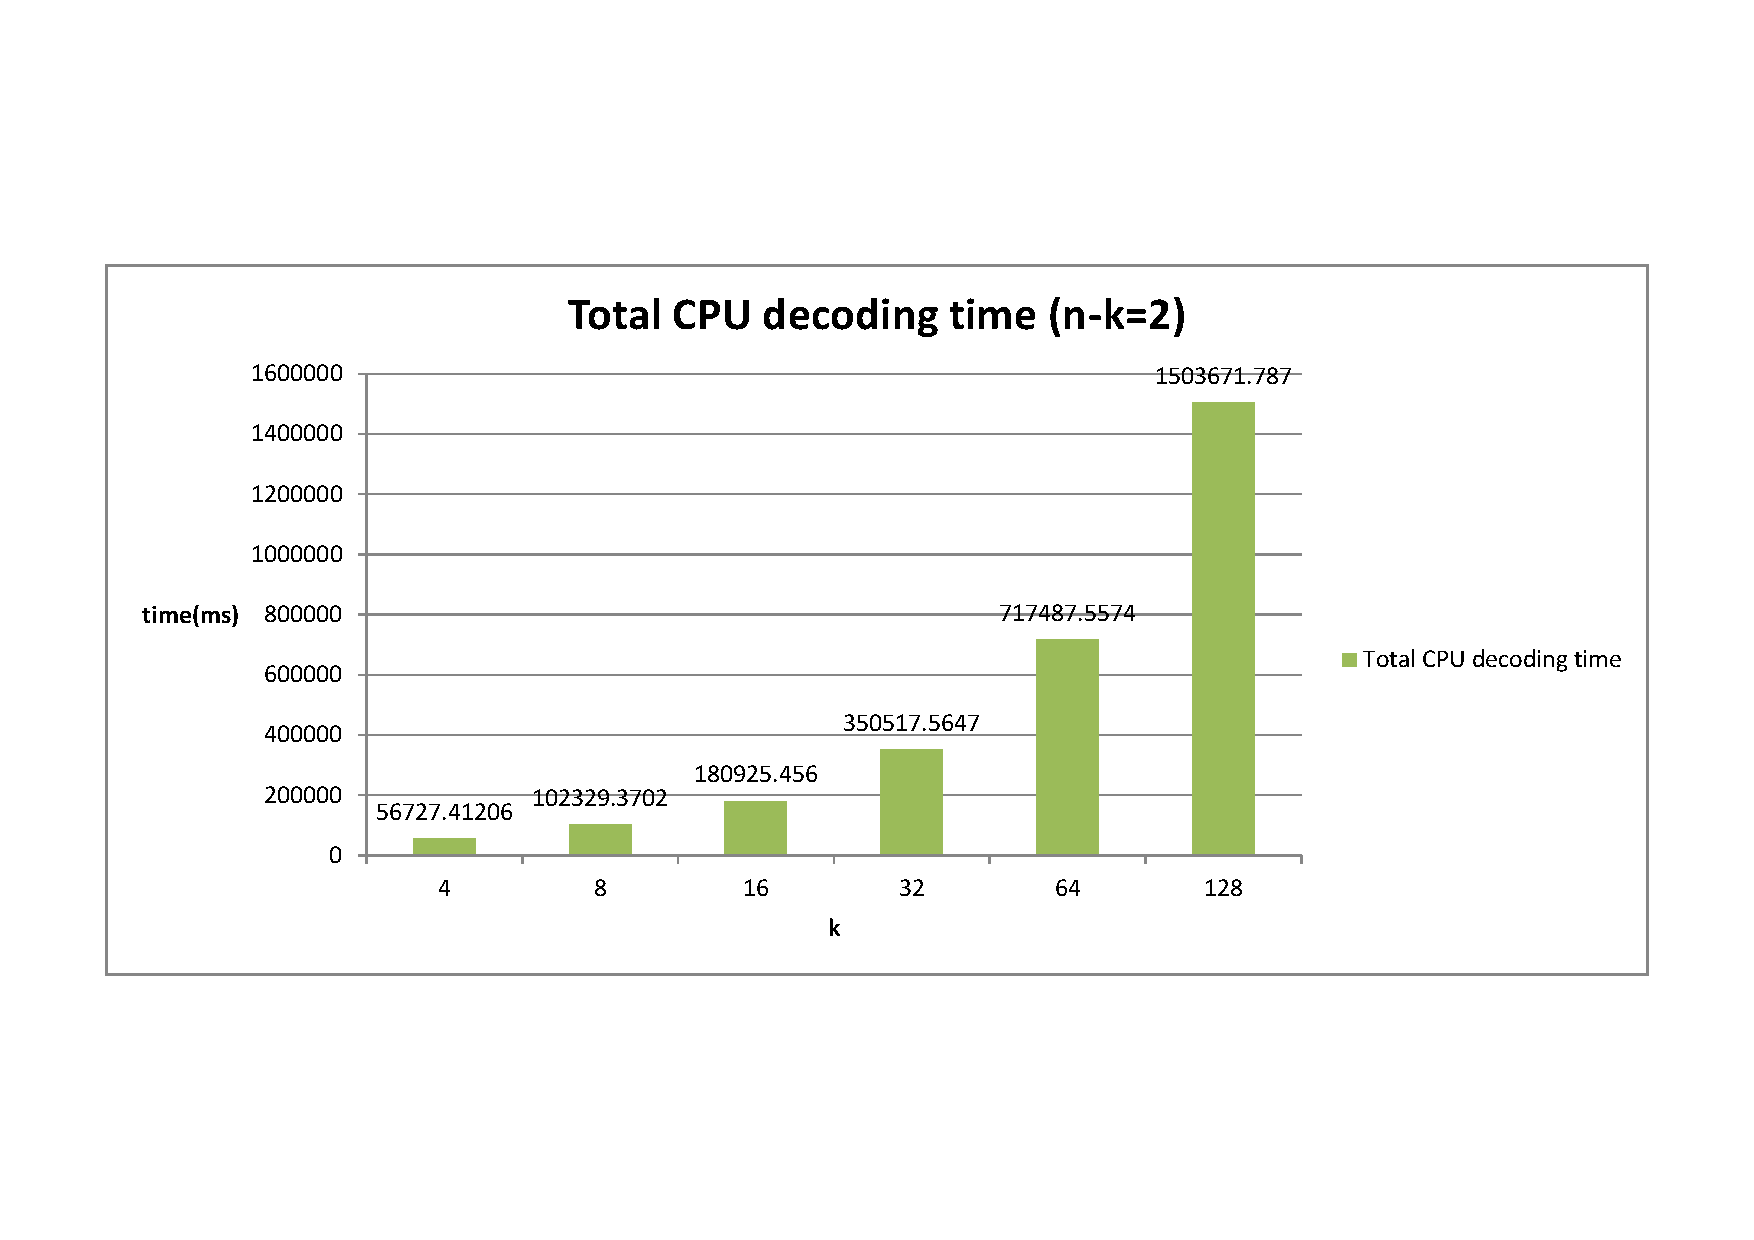
\includegraphics[scale=0.42]{../result-graph/Total-CPU-decoding-time-2.pdf}
}
\only<5>
{
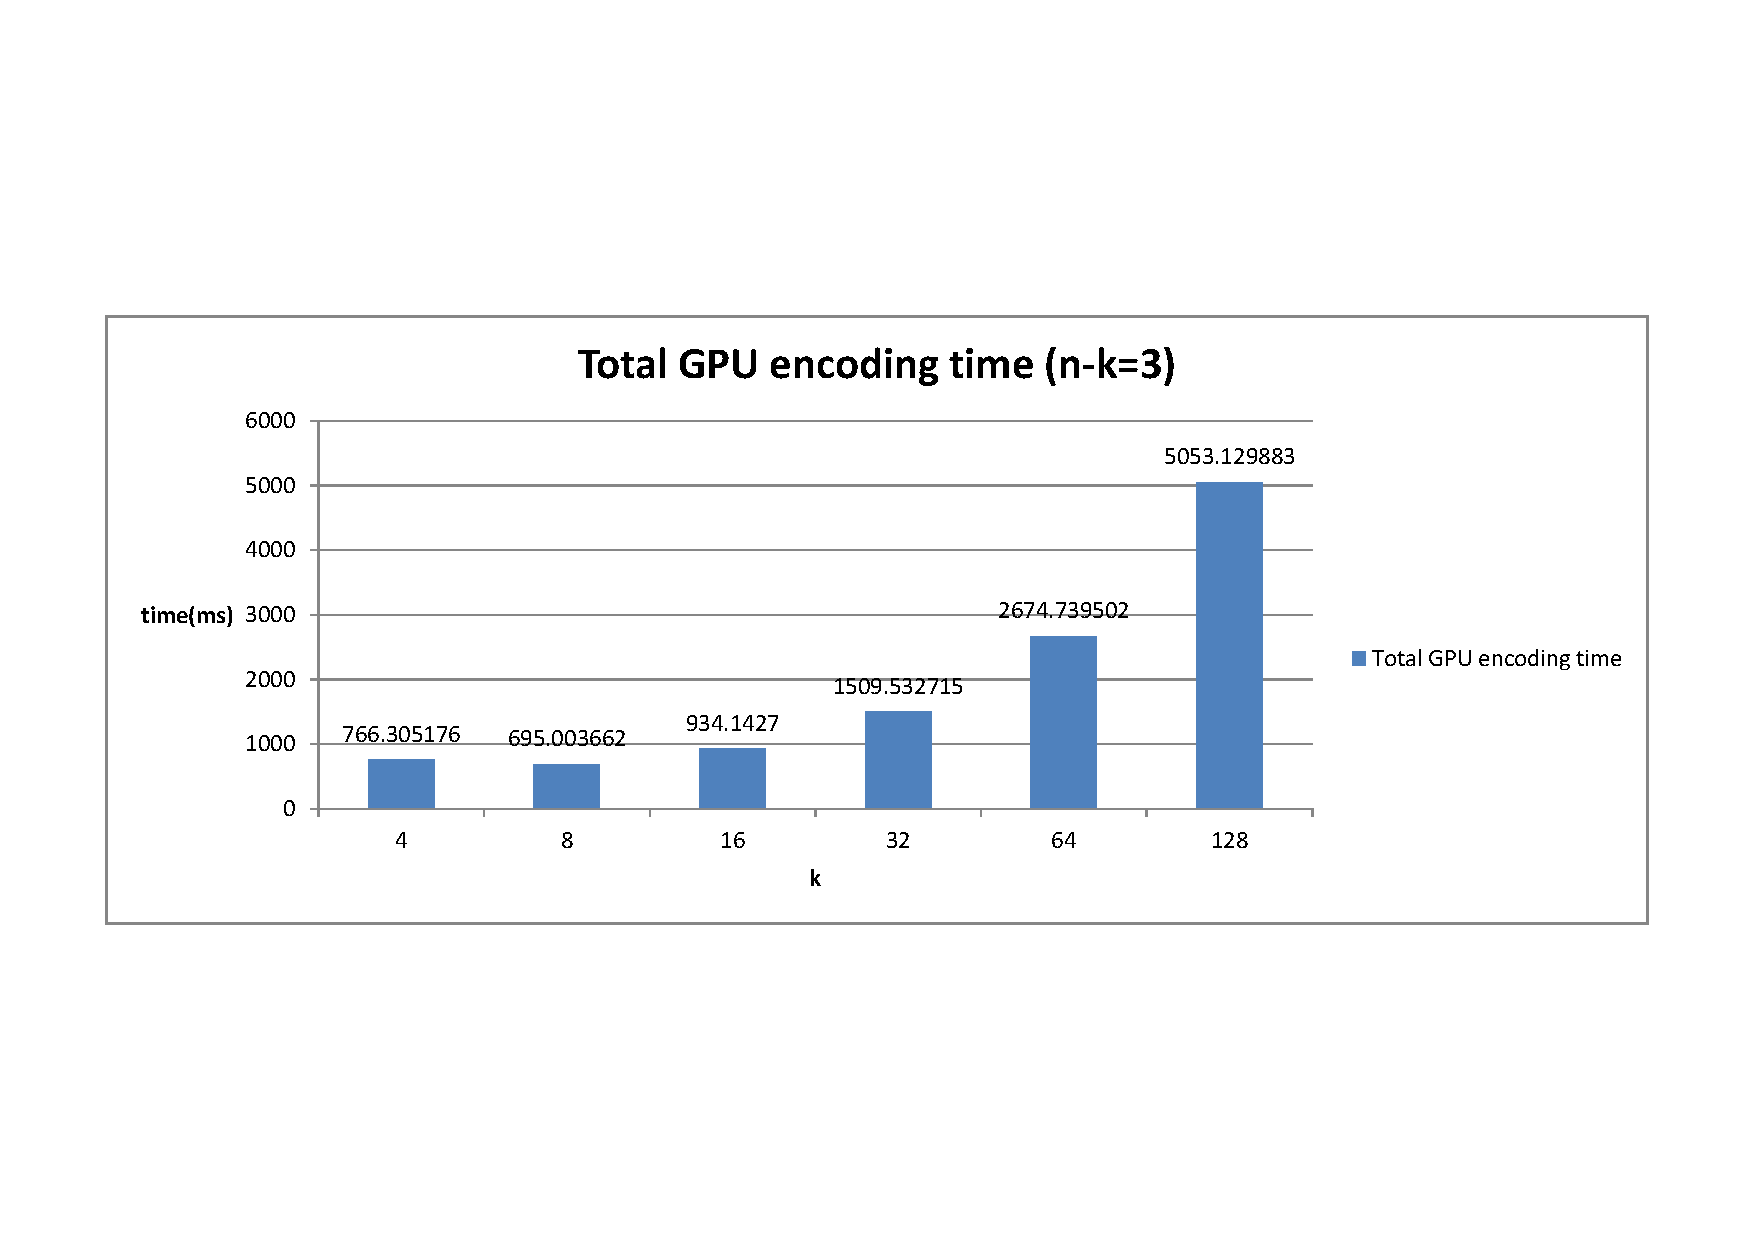
\includegraphics[scale=0.42]{../result-graph/Total-GPU-encoding-time-3.pdf}
}
\only<6>
{
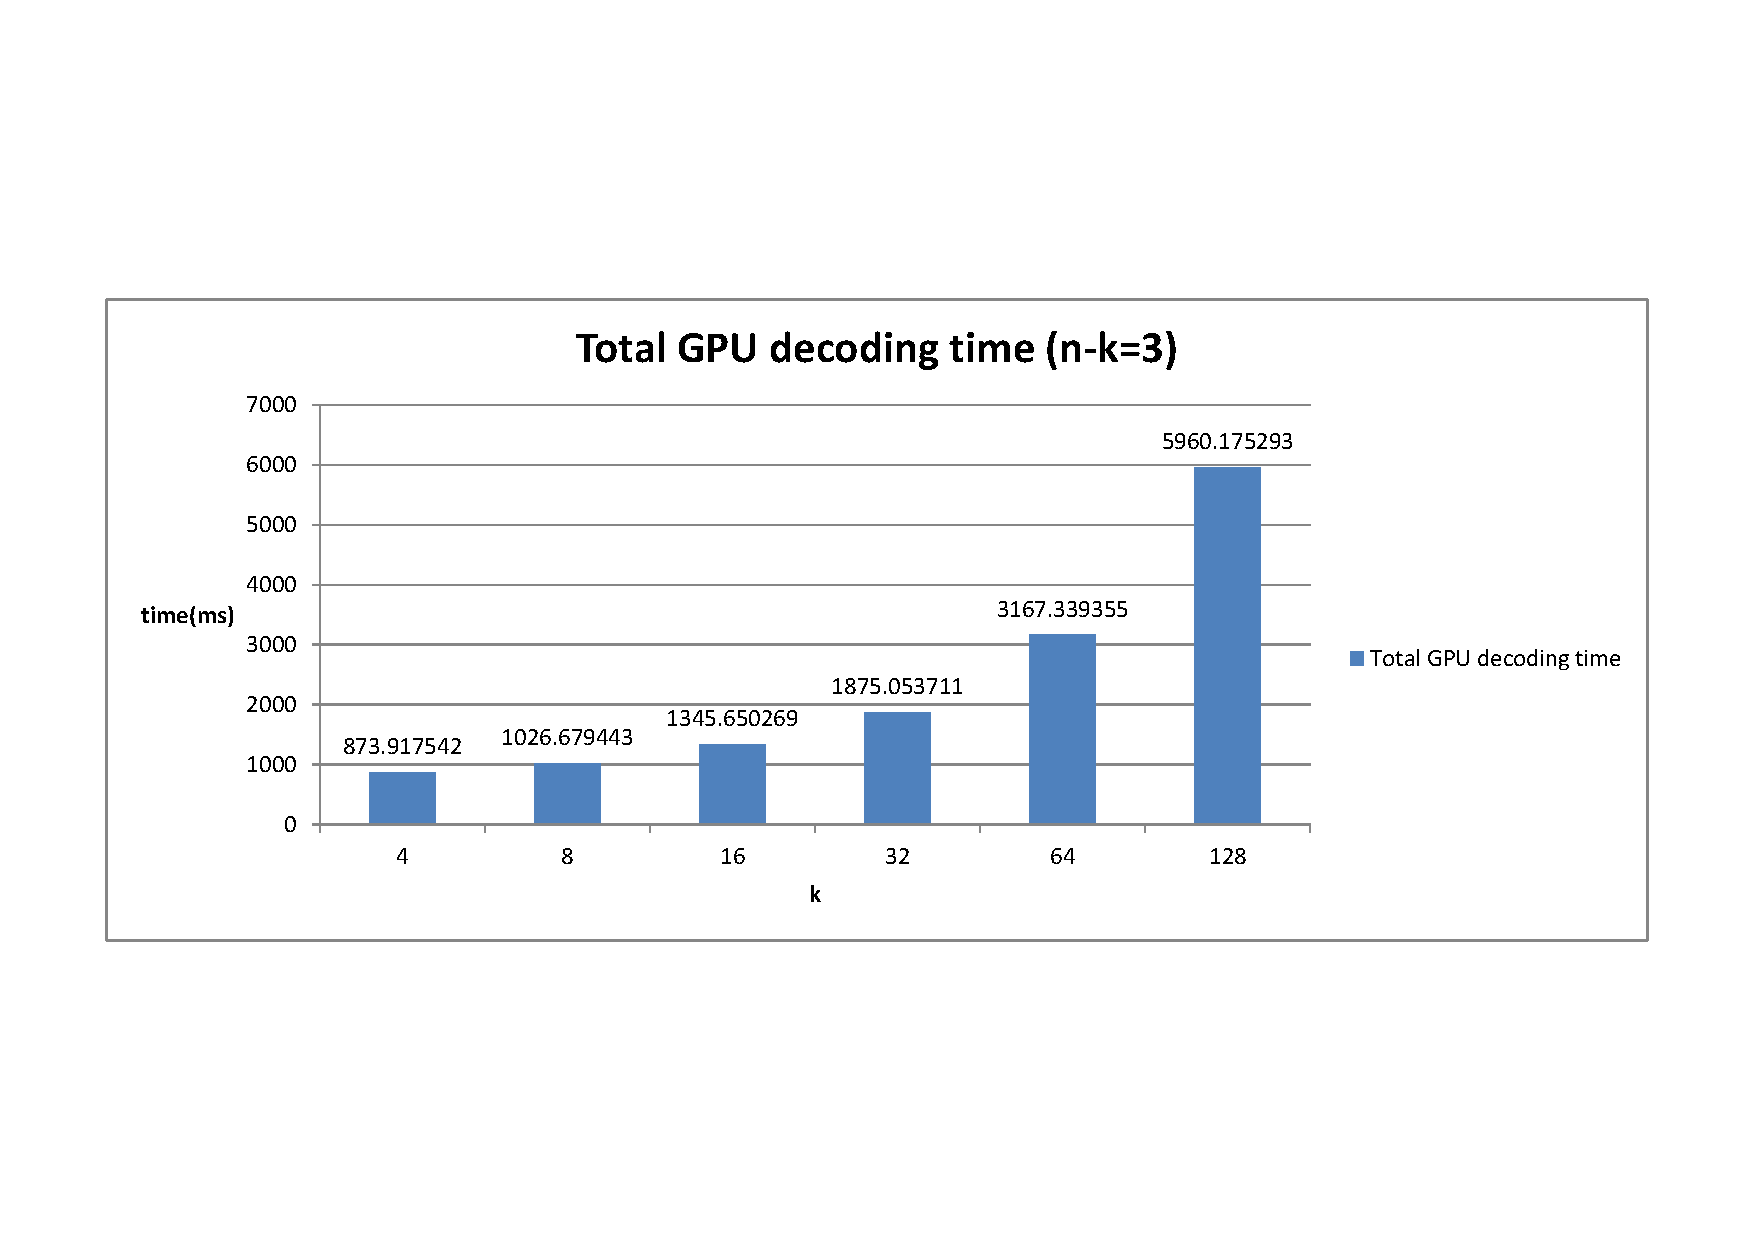
\includegraphics[scale=0.42]{../result-graph/Total-GPU-decoding-time-3.pdf}
}
\only<7>
{
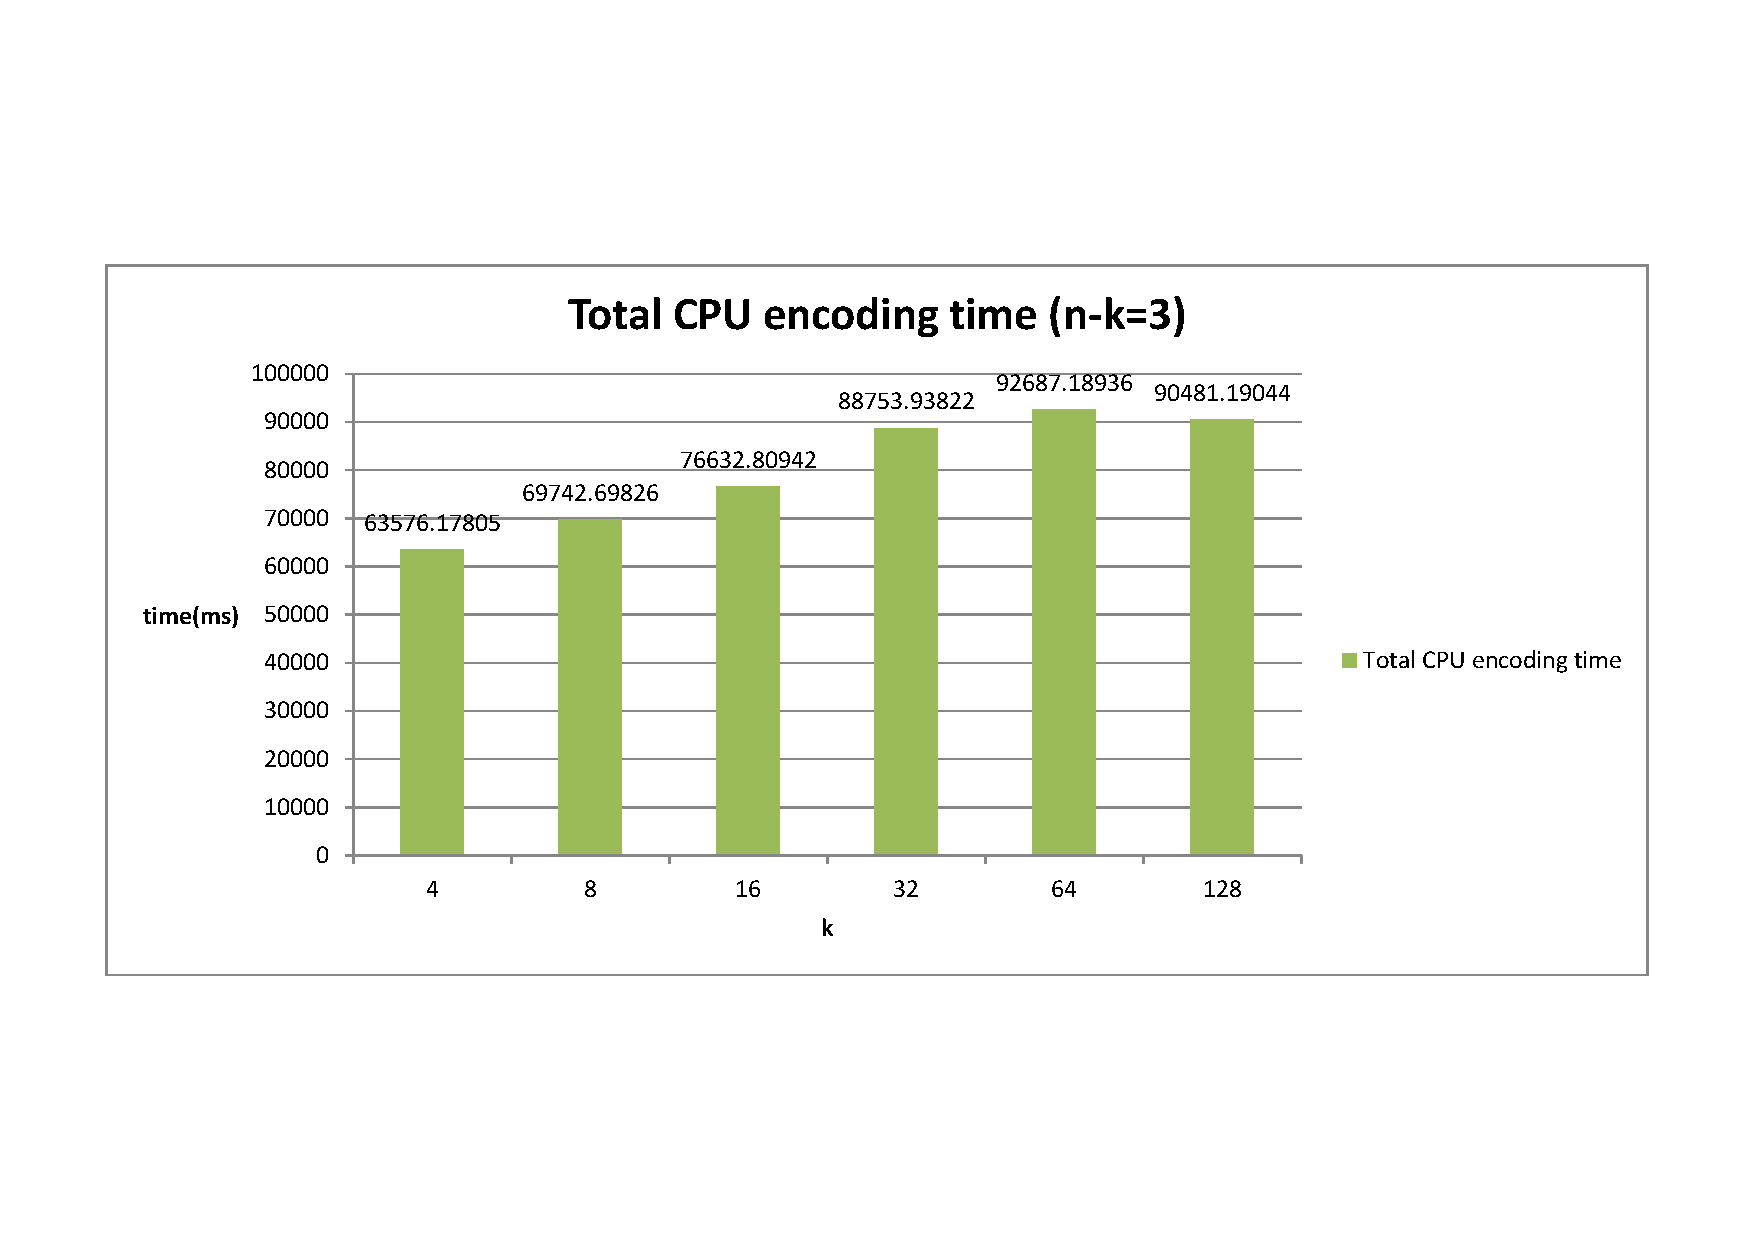
\includegraphics[scale=0.42]{../result-graph/Total-CPU-encoding-time-3.pdf}
}
\only<8>
{
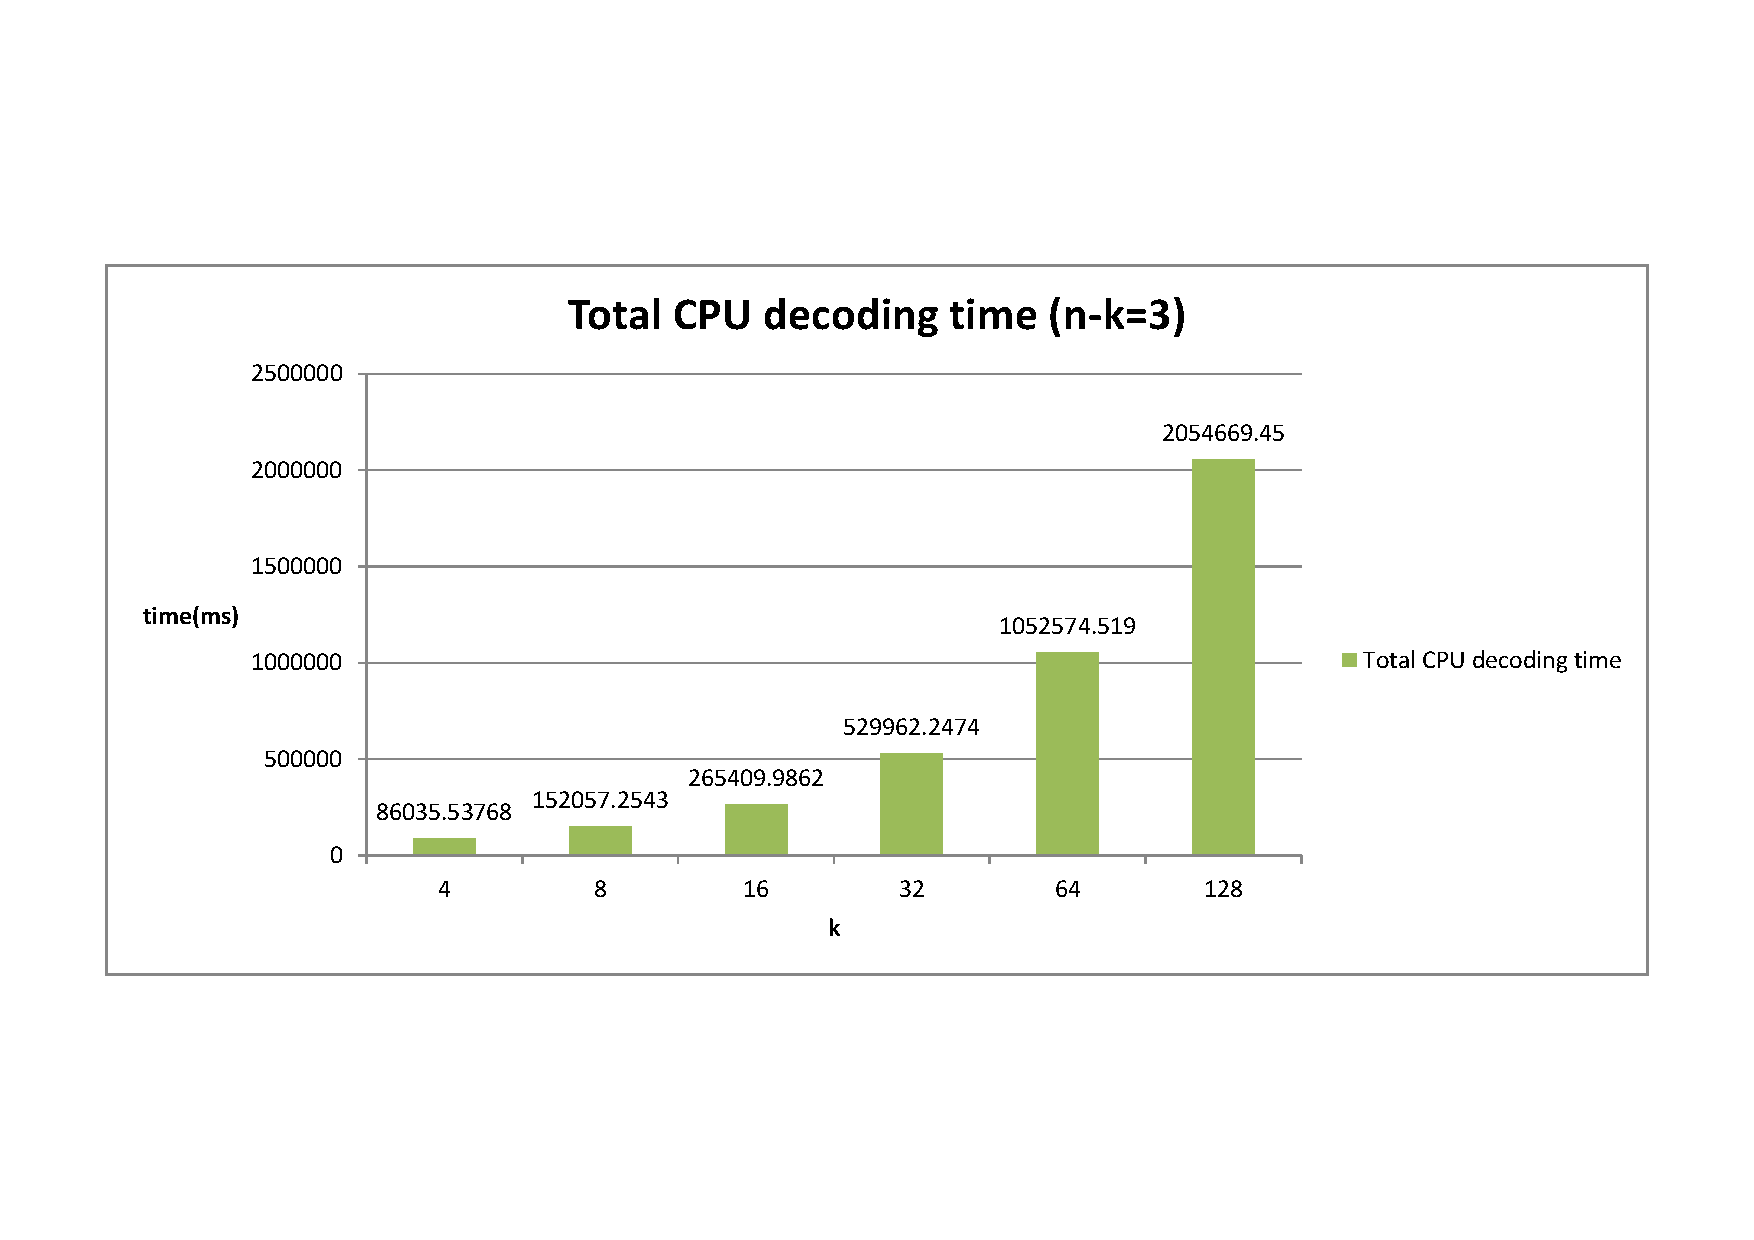
\includegraphics[scale=0.42]{../result-graph/Total-CPU-decoding-time-3.pdf}
}
\only<9>
{
\begin{block}{Conclusion}
\begin{enumerate}
\item If we divide the original data into more fragments (i.e. increasing $k$), we can achieve less storage overhead, meanwhile both CPU and GPU performance will become worse.
\item In reality, we seldom cut the files into more than 30 fragments, so the overall performance of GPU would still be acceptable.
\end{enumerate}
\end{block}
}
\end{frame}

\subsection{Experiment Result (GPU cost breakdown)} % Bookmark information
\begin{frame}[options]
\frametitle{Experiment Result (GPU cost breakdown)}
\only<1-4>
{
$k = 4, n = 6$
}
\only<1>
{
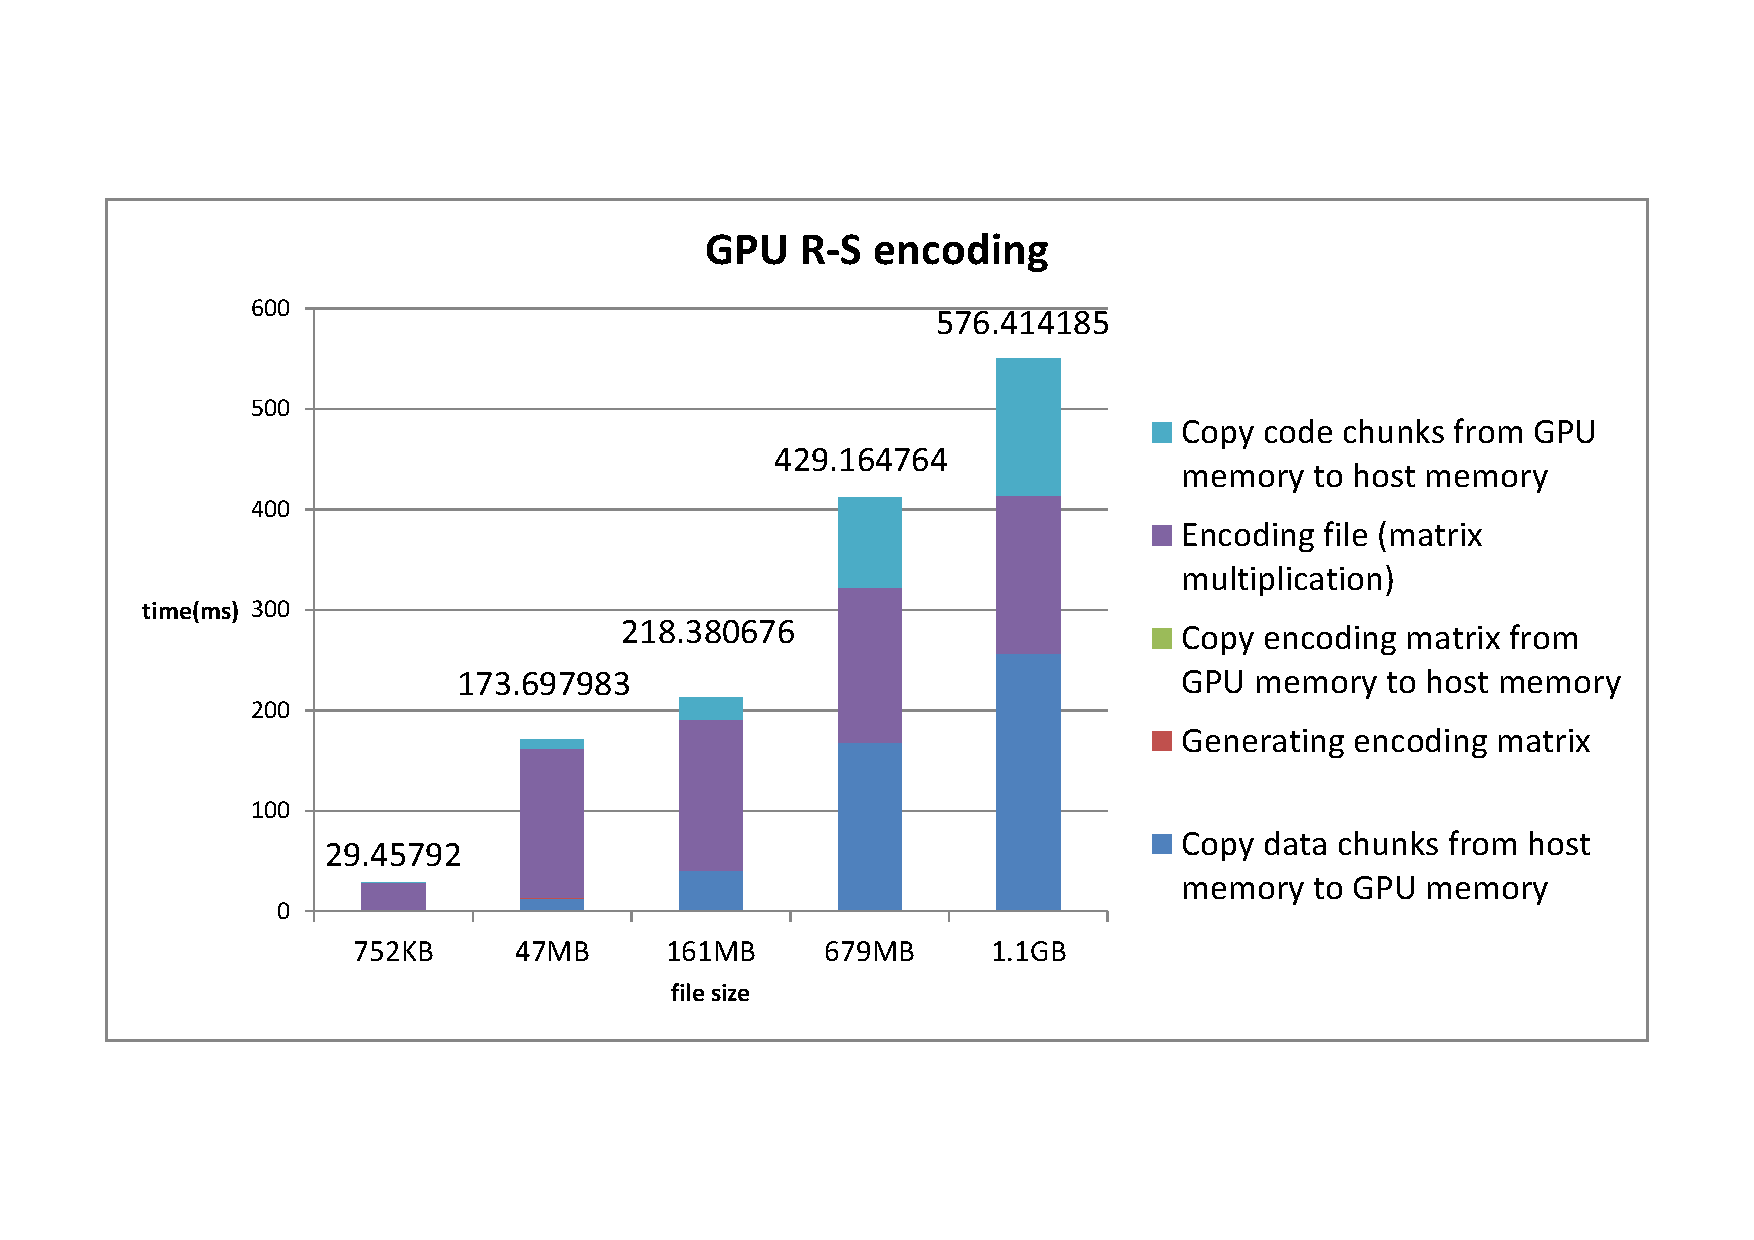
\includegraphics[scale=0.42]{../result-graph/GPU-encode-steps.pdf}
}
\only<2>
{
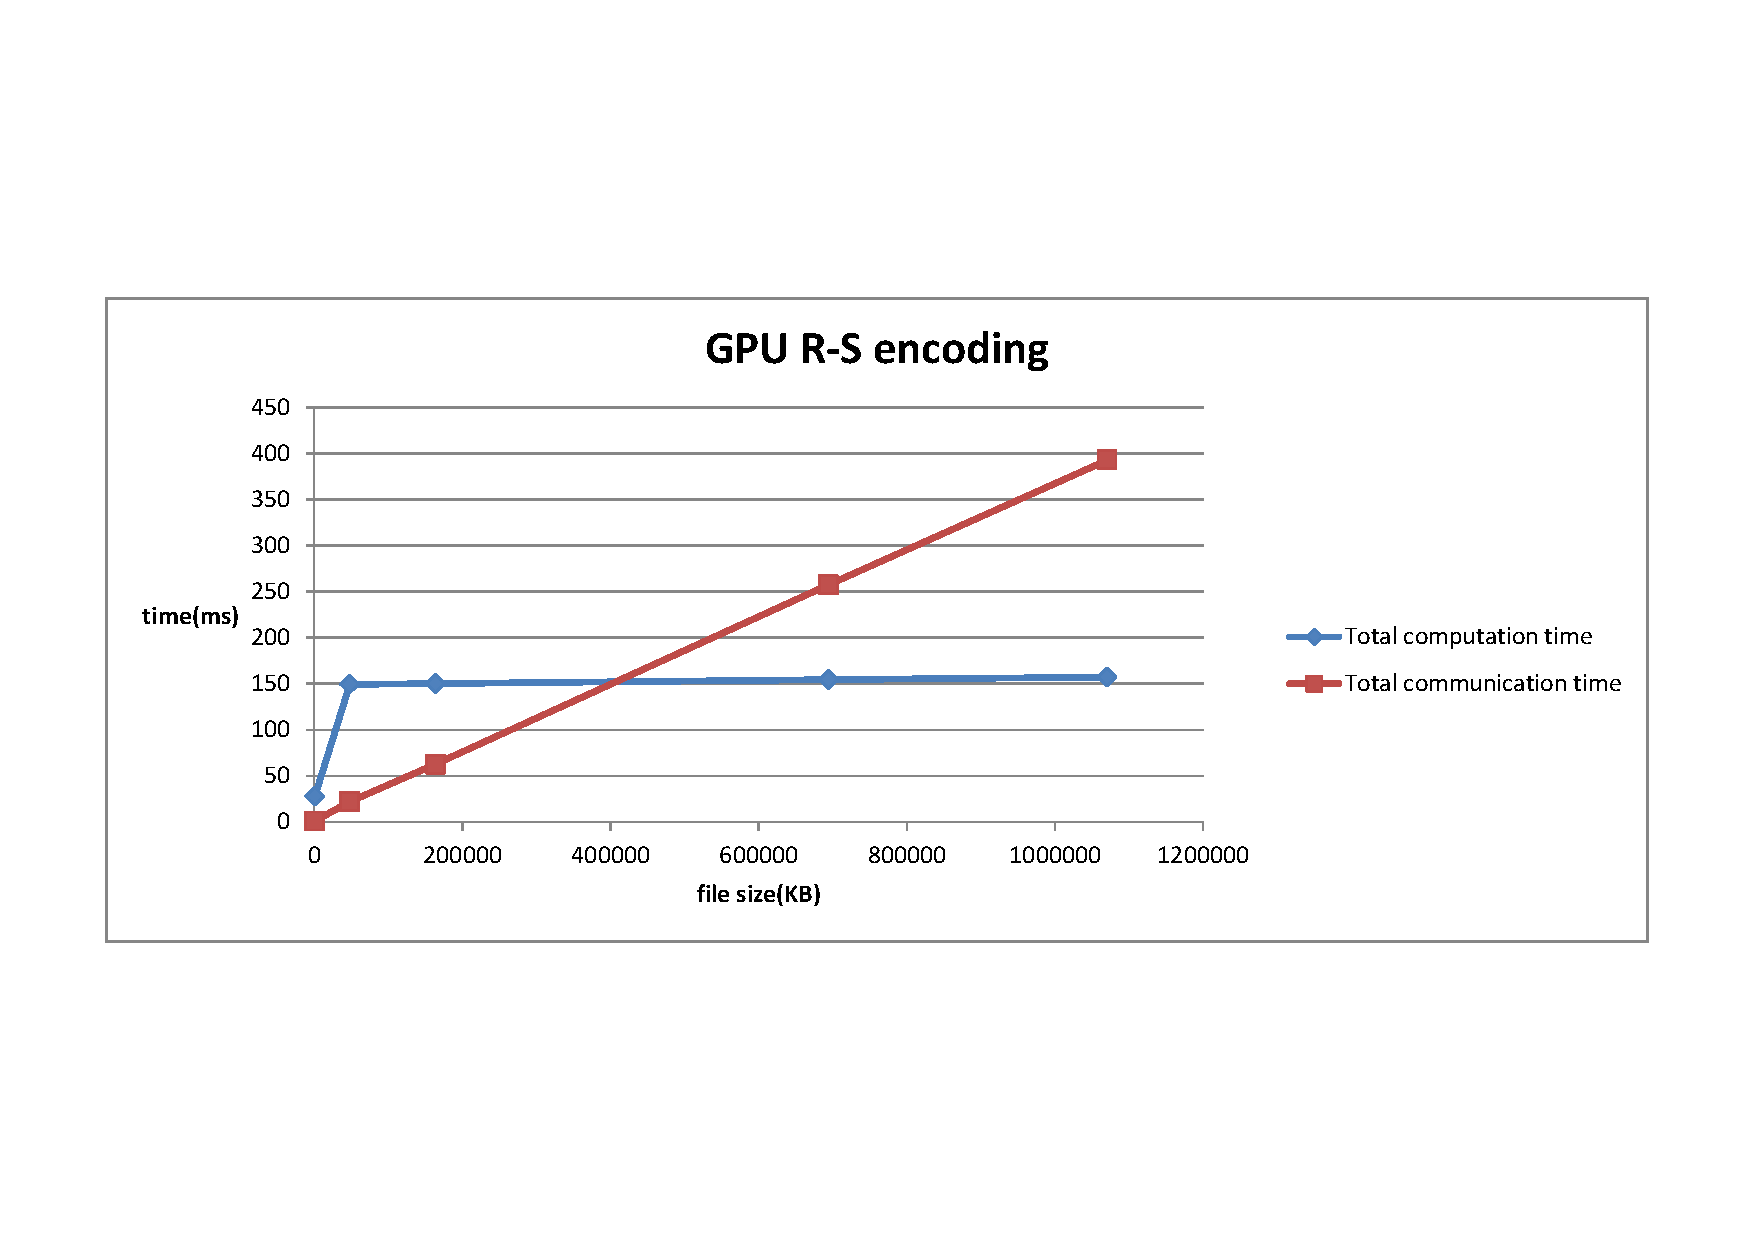
\includegraphics[scale=0.42]{../result-graph/GPU-RS-encode.pdf}
}
\only<3>
{
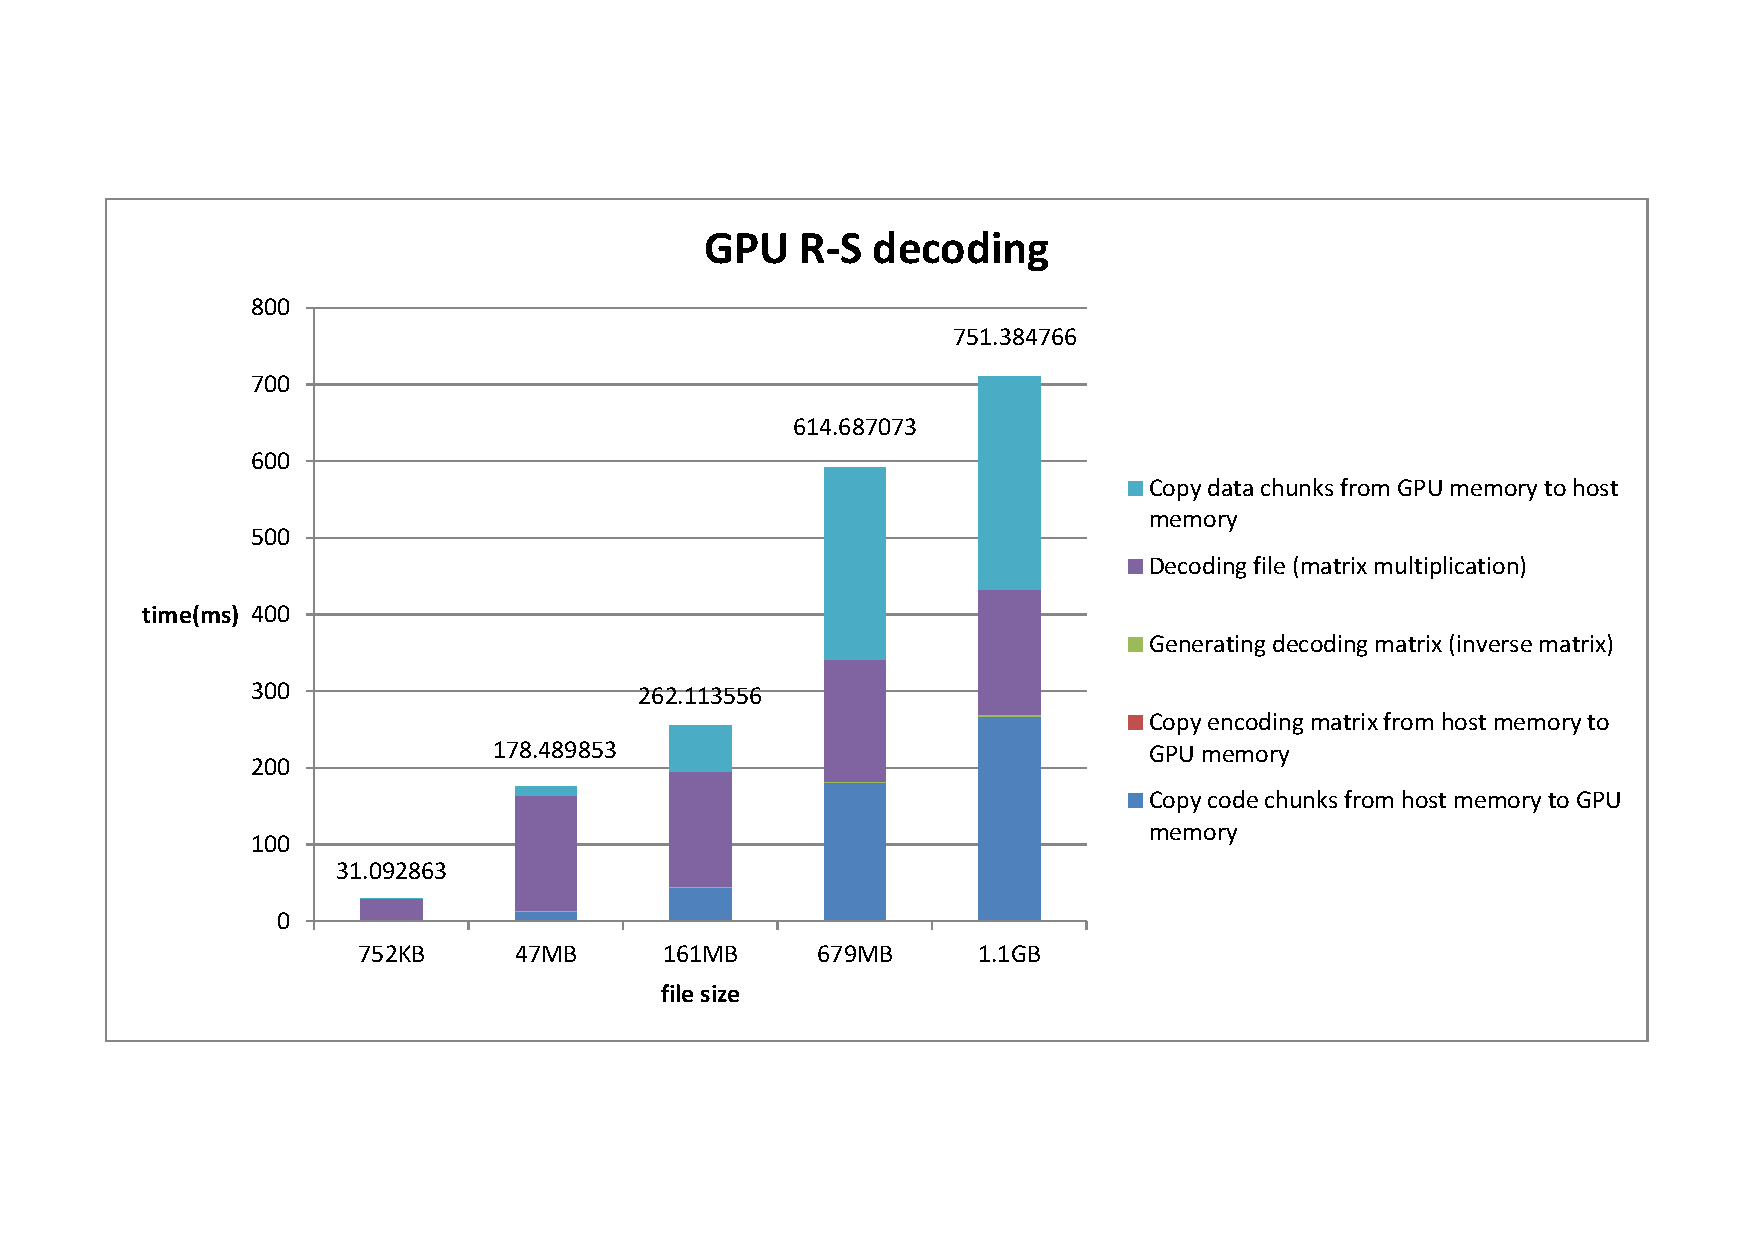
\includegraphics[scale=0.42]{../result-graph/GPU-decode-steps.pdf}
}
\only<4>
{
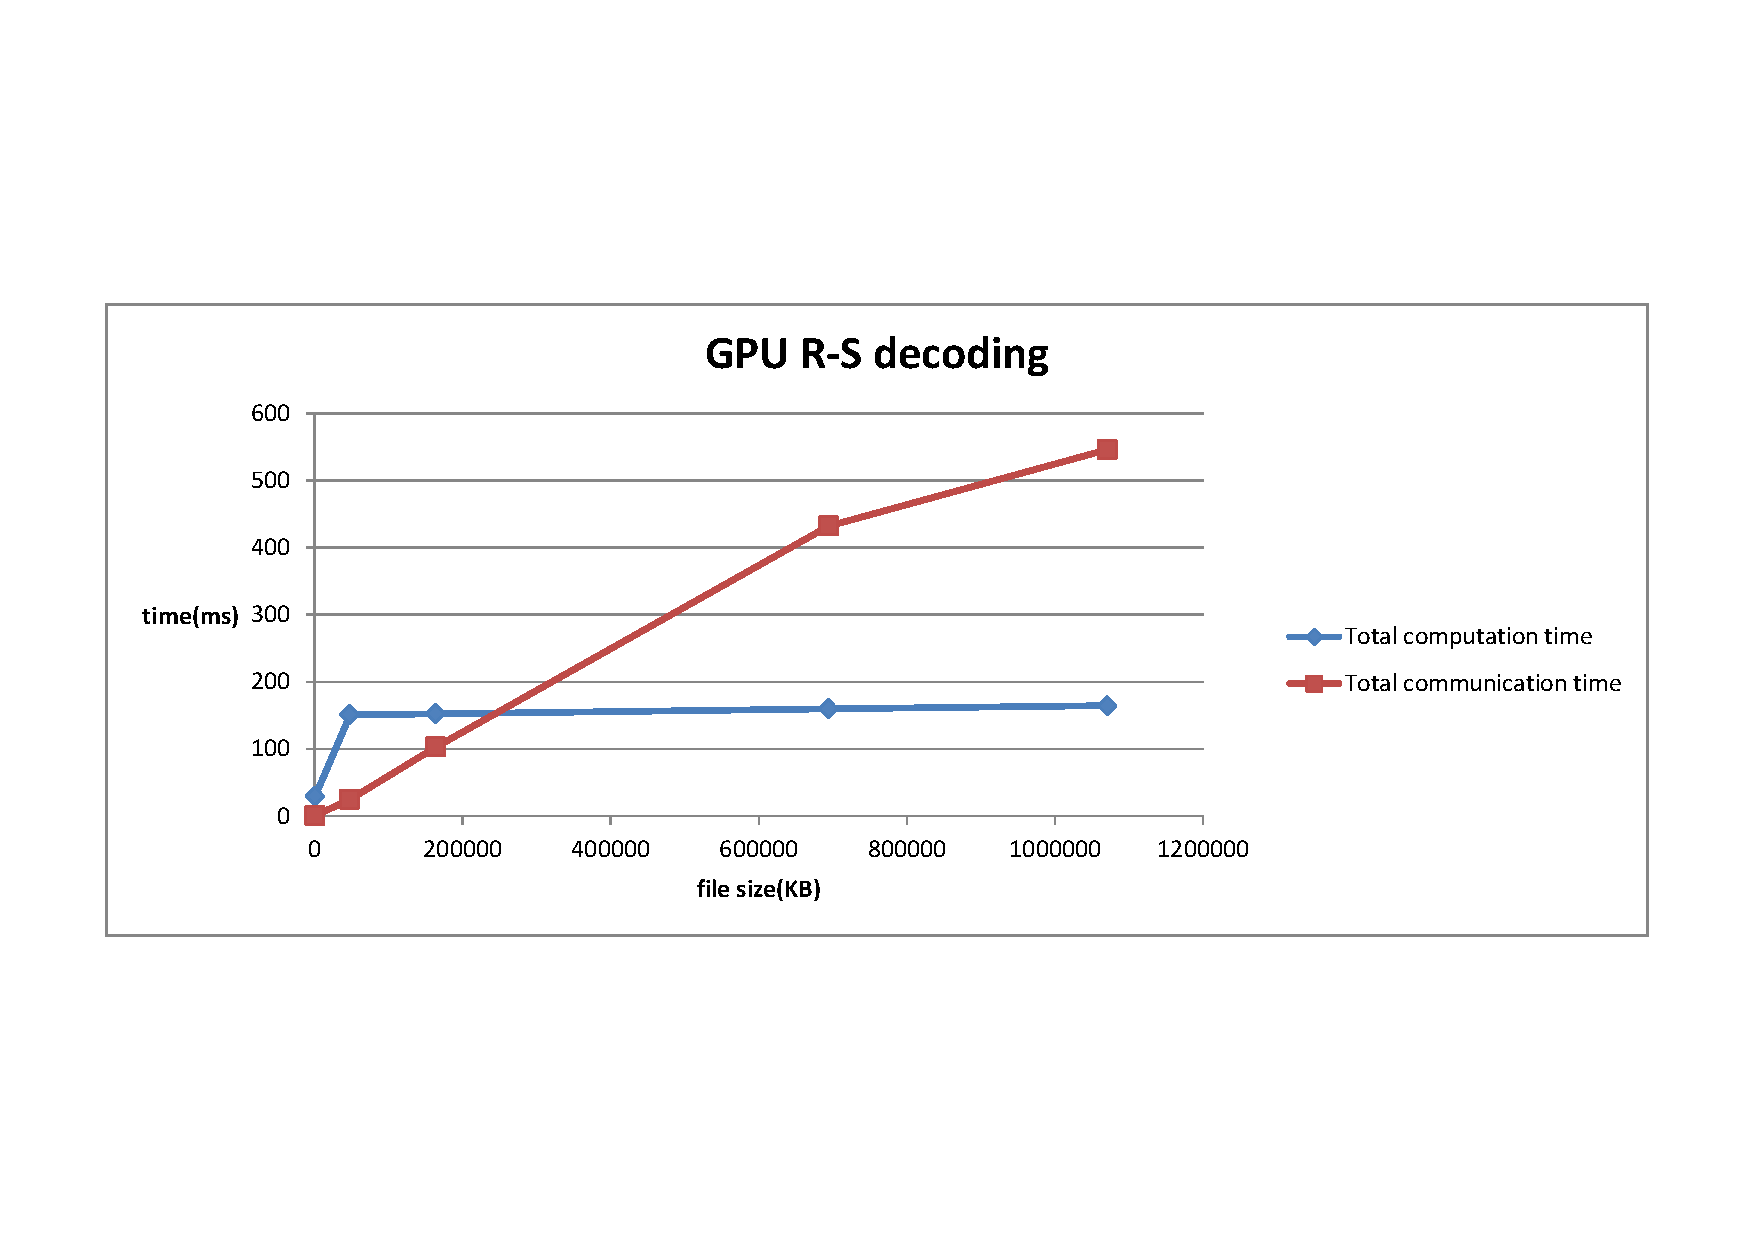
\includegraphics[scale=0.42]{../result-graph/GPU-RS-decode.pdf}
}
\only<5>
{
\begin{block}{Conclusion}
\begin{enumerate}
\item GPU computation time becomes almost constant when the file size is large enough.
\item Matrix multiplication time occupies much more percentage than matrix generation time in the breakdown of GPU computation time.
\item GPU spends more time in communication and the communication time is getting more as the file size becomes larger. This phenomenon explains why GPU performance speed-up gets slower.
\end{enumerate}
\end{block}
}
\end{frame}

\section{Q \& A} % Bookmark information
%\subsection{Conclusion} % Bookmark information
\begin{frame}[options]
\frametitle{Q \& A}
      \begin{center}
        Thank You!
      \end{center}
\end{frame}

\bibliographystyle{plain}
\bibliography{slide.bib}
\end{document}



